\chapter{BAYESIAN SHRINKAGE ESTIMATION OF LOGISTIC SMOOTH TRANSITION AUTOREGRESSIONS}
\label{chap:temp}

\section{Introduction}
Occasionally, classical linear time series models inadequately capture temporal dynamics in the expected levels of a process, resulting in suboptimal forecasting performance \citep{Lee1993}. The presence of significant nonlinear associations leads to the daunting task of selecting an adequate model from an expanding library of nonlinear specifications. A parametric subset from the aforementioned library extends autoregressive processes to account for changes in regimes or states \citep{Priestley1988}; nonlinear phenomena in financial and economic time-series motivated the majority of research in this area \citep{Terasvirta2010,Zivot2006,Franses2000}. For example, asymmetries in quarterly national industrial production indexes can be explained by differentiating dynamics in two regimes: recessions and expansions \citep{Terasvirta1992}. Although popularized by econometricians, regime-switching nonlinear time series models have been applied in a variety of research problems related for instance to the dynamics of network flows \citep{Kamarianakis2010} and the dynamics of air \citep{Battaglia2012} and stream-water temperatures \citep{Kamarianakis2016}. 

In what follows, the univariate time series of interest is denoted by $y_t$. Let $\bm{x}'_t=[1,y_{t-1},y_{t-2}, \cdots, y_{t-p}]$, $\bm{\alpha}=[\alpha_0,\alpha_1,\cdots,\alpha_p]$ and $\bm{\beta}=[\beta_0,\beta_1,\cdots,\beta_p]$. A parametric regime-switching time series model is formulated as:
\begin{equation}
\label{eq:1}
y_t=(\bm{x}'_t\bm{\alpha})(1-G(z_{t},\gamma,\delta))+(\bm{x}'_t\bm{\beta})G(z_{t},\gamma,\delta)+\epsilon_t \textrm{ where } \epsilon_t \sim \textrm{i.i.d. } N(0,\sigma^2)
\end{equation}
If $0\leq G(z_{t},\gamma,\delta) \leq 1$, Equation \ref{eq:1} represents a weighted average of two autoregressive processes of order $p$ (AR(p)), with weights depending on the value of the transition variable $z_t$. When $z_t=y_{t-d}$ the model is a ``self-exciting autoregression'' and an additional delay parameter $d$ is introduced \citep{Petruccelli1984}. Equation \ref{eq:1} represents a logistic smooth transition autoregressive model of order $p$ (LSTAR(p)) when $G(y_{t-d},\gamma,\delta)=\{1+\exp[-(\gamma/s_y)(y_{t-d}-\delta)]\}^{-1}$. If $y_{t-d} < \delta$, $G(y_{t-d},\gamma,\delta) < 1/2$ and the AR(p) model $\bm{x}'_t\bm{\alpha}$ in the ``low regime'' is favored, whereas when $y_{t-d} > \delta$, $G(y_{t-d},\gamma,\delta) > 1/2$ and the AR(p) model $\bm{x}'_t\bm{\beta}$ in the ``high regime'' receives larger weights. The slope $\gamma$ determines the speed of transition between regimes; scaling $\gamma$ by the sample standard deviation of the transition variable $s_y$ allows for scale-free comparisons across competing STAR models with differing  transition variables \citep{Deschamps2008}. As $\gamma \to \infty$,  $G(y_{t-d},\gamma,\delta) \to \mathbbm{1}_{\{y_{t-d}>\delta\}}(y_{t-d})$ that evaluates to $1$ if $y_{t-d}>\delta$ and $0$ otherwise. Hence, in the limiting case when regime changes are abrupt, Equation \ref{eq:1} is equivalent to a threshold autoregressive model of order $p$ (TAR(p)). Although this work focuses on the homoskedastic case, it is not hard to fathom the variance of $y_t$ exhibiting regime switching dynamics along with the mean of $y_t$. Most research regarding STAR models revolves around the two regime case; however, extensions have been made to account for multiple ($>$2) regimes (MR-STAR) \citep{Terasvirta2010}. 

Bayesian estimation of two-regime LSTAR(p) models was initially developed by \citep{Lubrano2000}. \citep{Lopes2006} expanded Lubrano's methodology to include the model order $p$ in the vector of unknown parameters, using the reversible jump markov chain monte carlo (RJMCMC) algorithm presented in \cite{Green1995}. These changes were inspired by \citep{Troughton1997} who applied RJMCMC to AR(p) models. Further work by \citep{Gerlach2008} accounted for regime-specific heteroskedasticity. Current Bayesian estimation methods of the LSTAR(p) typically assume that the autoregressive order $p$ is the same in both regimes and estimate coefficients corresponding to all autoregressive terms $y_{t-k}$ for $k \in \{1,2,...,p\}$. If the true nonlinear data generating process (DGP) has regime-specific orders with some autoregressive terms being non-significant, the above-mentioned method is expected to be suboptimal in terms of out-of-sample predictive accuracy as it is not flexible enough to capture the data generating process. 

Section 2 explains how Bayesian estimation methods for sparse signals can be incorporated in the sampling algorithm for LSTAR models and how a $Dirichlet$ prior may be used to estimate a generalized variant of the transition function. The proposed methodology is an alternative to existing stepwise model building strategies and to RJMCMC schemes: it estimates in a single step, specifications which encompass LSTAR and it may identify complex data generating mechanisms in which the values of transition function are determined by more than one threshold variable. Section 3 provides results from a series of Monte Carlo experiments showing the efficacy of the proposed methods. Section 4 presents a forecasting exercise based on benchmark data analyzed extensively in previous studies. Section 5 gives a positive outlook on how these methods may further advance Bayesian estimation of more complicated nonlinear processes and the last Section concludes the paper.


%%%%%%%%%%%%%%%%%%%%%%%%%%%%%%%%%%%%%%%%%%%%%%%%%%%%%%%%%%%%%%%%%%%%%%%

\section{Methodology}

\subsection{Bayesian Estimation of LSTAR}
 For the 2-regime LSTAR(p) model in Equation \ref{eq:1} define the full vector of unknown parameters $\bm{\theta}=[\alpha_0, \alpha_1, \cdots, \alpha_p, \beta_0,\cdots,\beta_p, \gamma,\delta,\sigma,d,p]'$ where $\gamma=\gamma^*/s_y$. In regards to $\bm{\alpha}$, $\bm{\beta}$, and $\sigma^2$, the prior specifications presented in previous research works are  $\alpha_k \sim N(\mu_\alpha,\sigma^2_\alpha)$, $\beta_k \sim N(\mu_\beta,\sigma^2_\beta)$, $1/\sigma^2 \sim IG(a_{\sigma^2},b_{\sigma^2})$, where $N$ and $IG$ respectively denote normal and inverse-gamma distributions. To ensure that sufficient representation exists in both regimes, the prior for $\delta$ is defined as $\delta \sim U[q_Y(0.15),q_Y(0.85)]$, where $q_Y(.)$ is the empirical quantile function of the observed transition variable and $U[a,b]$ represents the uniform distribution bounded on  $[a,b]$. Using the $15^{th}$ and $85^{th}$ percentiles ensures that at least 15\% of the data belongs to each regime. The parameter $d$ is typically given a discrete uniform prior $P(d=\tilde{d})=1/d_{max} \textrm{ for } \tilde{d} \in \{1,2,\cdots,d_{max}\}$, where $d_{max}$ is chosen \textit{a priori}.
 
Difficulties in the estimation of $\gamma=\gamma^*/s_y$ have led to a variety of prior proposals: $Cauchy$ \citep{Lubrano2000},  $Gamma$ \citep{Lopes2006}, $truncated-Normal$ \citep{Livingston2017}, and $log-Normal$ \citep{Gerlach2008}.  \cite{Livingston2017} compared  $Gamma$ and $truncated-Normal$ and demonstrated that computational time and posterior results are mainly influenced by starting values and prior information rather than distributional choice. \cite{Gerlach2008} favored the $log-Normal$ ($LN$) prior $\gamma^* \sim LN(\mu_\gamma,\sigma^2_\gamma)$ over $Cauchy$, since it leads to an integrable posterior for $\gamma$ and removes unnecessary prior weight placed at 0. Our preliminary analyses showed that the choice of prior had little effect on posterior distributions, confirming the findings by \cite{Livingston2017}. In what follows, $log-Normal$ priors are adopted for $\gamma^*$ since it resulted in low computational times relative to $Gamma$, $Cauchy$ and $truncated-Normal$.
 
Sampling algorithms of the joint posterior $f(\bm{\theta}|\bm{y})$ exploit that the LSTAR($p$) model is conditionally linear given $\gamma^*$ and $\delta$. Specifically, Gibbs sampling is applied for $\bm{\alpha}$, $\bm{\beta}$, and $\sigma^2$  \citep{Gelfand1990} and Metropolis-Hastings \citep{Metropolis1953,Hastings1970} for $\gamma^*$ and $\delta$. Since the length of $\bm{\theta}$ increases with the model order $p$, \cite{Lopes2006} extended the sampling algorithm outlined by \cite{Lubrano2000} to incorporate a reversible jump step, which includes the model order $p$ in $\bm{\theta}$. RJMCMC allows the dimension of the sampled vector $\bm{\theta}$ to change from $2(p+1)+3$ to $2(p'+1)+3$ whenever proposed changes from $p$ to $p'$ are accepted. Posterior assessment with regard to $p$ relies on comparing  posterior model probabilities. The most likely model order $\hat{p}$ is defined as $\hat{p}=\max_{p}\#\{p_s=p| s \in {1,\cdots, S}\}/S$  where $S$ represents the number of samples from the joint posterior distribution after burn-in and $p_s$ represents the sampled value at iteration $s$. 

\subsection{Sparse Estimation via Bayesian Shrinkage}
Let $p_1$ be the true linear AR model order in the low regime and $p_2$ be its equivalent in the high regime. Furthermore, let $p=\max\{p_1, p_2\}$. Two cases where RJMCMC may never sample from the correct parameter space are when $p_1\neq p_2$ or when $\exists \textrm{ } j <p$ such that $\alpha_j=0 \cup \beta_j=0$. The conditional linear nature of the LSTAR(p) model invites a plethora of Bayesian techniques for model selection through the editing of the priors for $\bm{\alpha}$ and $\bm{\beta}$. For insights into the different varieties, the interested reader may consult \cite{OHara2009}. 

Stochastic search variable selection (SSVS) builds a mixture of two normal distributions centered at 0, one with small variance and one with large variance, using indicator variables as the mixing weights \citep{George1993}. As different subsets of predictors are identified, coefficients of non-significant predictors are drawn toward 0 by the conditional nature of the priors in SSVS. Adaptive shrinkage methods, that achieve sparsity by using priors represented as scale mixtures of normal distributions, are shaped similarly to SSVS. An expanding list of hierarchical prior representations incorporates tuning parameters to perform shrinkage, by manipulating the amount of prior mass at zero and the shape of the tails \citep{Polson2010}. These methods are Bayesian analogs to penalized (regularized) estimates \citep{Tibshirani1996}, which have been employed to estimate linear time series models \citep{Konzen2016,Nardi2011}. 

Once a maximum order $p$ is specified \textit{a priori}, Bayesian shrinkage provides a flexible model building alternative; unlike RJMCMC, LSTAR(p) estimation can be performed using popular Bayesian software such as JAGS \citep{Plummer2003}. Furthermore, these methods may be applied to all models expressible by Equation \ref{eq:1}, including exponential smooth transition autoregressive (ESTAR) and TAR models. Future discussion is limited to four prior hierarchical representations, varying in shrinkage flexibility.

\subsubsection{Bayesian LASSO (BLASSO)}
\cite{Andrews1974} demonstrated that the double-exponential distribution can be expressed as a scale-mixture of normal distributions. Their work leads to the two-level hierarchical representation depicted in Equation \ref{eq:lassoprior}, where $EXP$ denotes the $Exponential$ distribution.
\begin{equation}
	\label{eq:lassoprior}
	\begin{split}
	\alpha_j|\sigma^2,\tau^2_{\alpha_j} \sim N(0,\sigma^2\tau^2_{\alpha_j}) \textrm{,  }  \tau^2_{\alpha_j}| \sim EXP(\lambda^2/2)\\ 
	 \beta_j|\sigma^2,\tau^2_{\beta_j}\sim N(0,\sigma^2\tau^2_{\beta_j}) \textrm{,  } \tau^2_{\beta_j}| \sim EXP(\lambda^2/2)
	\end{split}
\end{equation}
The hyperparameter $\lambda$ controls shrinkage across both regimes. In a linear context, as $\lambda \to \infty$ the path of  posterior medians settles between the regularization paths under $L_1$ and $L_2$ penalties \citep{Park2008}; therefore, this method is often called Bayesian LASSO (BLASSO). In the LASSO of \cite{Tibshirani1996}, the tuning parameter $\lambda$ is chosen via generalized cross validation. Rather than selecting a fixed $\lambda$, Bayesian procedures update this hyperparameter as MCMC moves through the posterior distribution
\citep{George2000,Casella2001,Yuan2005} using a $Gamma$ hyperprior $\lambda^2 \sim G(a_\lambda,b_\lambda)$. The full Gibbs sampler outlined by \cite{Park2008} can be extended to the LSTAR($p$) model using a  Metropolis-Hastings scheme for parameters $\{\gamma^*, \delta\}$.

\subsubsection{Regime-Specific Bayesian LASSSO (RS-BLASSO)}
A regime-specific variant of BLASSO, named (RS-BLASSO), employs two regime-specific tuning parameters $\lambda_1$ and $\lambda_2$, with independent gamma hyperpriors. The motivation for using two shrinkage parameters arrives from the understanding that sparseness may differ between the two regimes. A later simulation will identify a situation where this added flexibility is necessary for convergence. The corresponding modification to the BLASSO hierarchy is shown in Equation \ref{eq:lassoprior2}. 
\begin{equation}
	\label{eq:lassoprior2}
	 \tau^2_{\alpha_j}| \sim EXP(\lambda_1^2/2) \textrm{,  } \tau^2_{\beta_j}| \sim EXP(\lambda_2^2/2)
\end{equation}

 \subsubsection{Variable Selection with Bayesian LASSO (VS-BLASSO)}
A popular Bayesian subset selection method for linear models uses independent \textit{Bernoulli} ($BERN$) distributed variables to indicate either inclusion or exclusion of a covariate \citep{Kuo1998}. \cite{Lykou2013} combined this subset selection method with the \textit{double exponential} ($DEXP$) priors of BLASSO (VS-BLASSO). The BLASSO of \cite{Yuan2005} also employs binary selection variables, but only in a SSVS context. Introducing latent binary variables $\zeta_j$ and $\eta_j$ for $j \in \{1,2,\cdots, p\}$, the autoregressive coefficients are reparamaterized to $\alpha_j=\zeta_j\alpha_j^*$ and $\beta_j=\eta_j\beta_j^*$ and the alternative prior hierarchy is seen in  Equation \ref{eq:lassoprior3}. The tuning parameter $\lambda$ handles global shrinkage, while the independent binary variables provide local variable selection. It is not unusual here for posterior medians of unnecessary parameters to be exactly zero. Combining these ideas opens the door to posterior comparisons of model probabilities and the easy incorporation of RJMCMC for faster convergence \citep{Dellaportas2002}.
\begin{equation}
\begin{split}
	\label{eq:lassoprior3}
	 \zeta_j \sim BERN(0.5) \textrm{,  } & \alpha_j^*|\sigma^2\sim DEXP\Big(0,\frac{\sigma^2}{\lambda}\Big) \\
	  \eta_j \sim BERN(0.5) \textrm{,  } & \beta_j^*|\sigma^2\sim DEXP\Big(0,\frac{\sigma^2}{\lambda}\Big)
\end{split}
\end{equation}

 \subsubsection{Bayesian Horseshoe (BHS)}
 
The horseshoe prior  of \cite{Carvalho2009} can also be expressed as a scale-mixture of normals. Along with a global shrinkage parameter $\lambda$, Bayesian horseshoe adds local shrinkage parameters $\lambda_{\alpha_j}$ and $\lambda_{\beta_j}$. This change allows finer discrimination between relevant and non-significant autoregressive parameters by preventing the simultaneous over-shrinking that may occur to the parameter space in BLASSO. The  Bayesian horseshoe (BHS) prior hierarchy described by \citep{Carvalho2010} is presented in Equation \ref{eq:hsprior} with $C^+$ denoting the \textit{half-Cauchy} distribution. Unfortunately, posterior sampling of $\alpha_j$ and $\beta_j$ does not compare to the ease of the Gibbs sampler for BLASSO since full conditional distributions cannot be found analytically; however, fast slice sampling methods have been developed \citep{Hahn2016,Hahn2018}.  
\begin{equation}
\begin{split}
	\label{eq:hsprior}
	\alpha_j|\lambda_{\alpha_j} & \sim N(0,\lambda_{\alpha_j}) \textrm{,  }  \beta_j|\lambda_{\beta_j} \sim N(0,\lambda_{\beta_j}) \\
	  \lambda_{\alpha_j} & \sim C^+(0,\lambda) \textrm{,  } \lambda_{\beta_j} \sim C^+(0,\lambda) \\
	  \lambda|\sigma^2 & \sim C^+(0,\sigma)
\end{split}
\end{equation}

\subsection{Estimating the Delay Parameter}

Till now, the delay parameter $d$ was assumed known as in \cite{Gerlach2008} whose focus was on regime-specific heteroskedasticity. However, this assumption is unreasonable in applications. The discrete uniform prior has been used for $d$ since \cite{Lubrano2000} and \cite{Lopes2006}. The discrete uniform prior restricts popular Bayesian MCMC software from incorporating the delay parameter in MCMC posterior sampling. This problem can be circumvented by building LSTAR specifications for a finite set of prospective values of $d$ and then choosing the model with the highest posterior probability \citep{Deschamps2008}. For model order $p$, one may consider all possible threshold variables $y_{t-d}$ for $d \in \{1,2, \cdots, p\}$; purposefully overestimating $p$ can lead to a tedious procedure for choosing the delay. 

Let $\bm{y}=[y_{t-1}, y_{t-2},\cdots,y_{t-p}]'$, $\bm{\phi}=[\phi_{1}, \phi_{2},\cdots,\phi_{p}]'$ and recall the transition function $G(z_t,\gamma,\delta)=\{1+\exp[-(\gamma^*/s_y)(z_t-\delta)]\}^{-1}$ in Equation \ref{eq:1}. A specification that nests LSTAR contains a new threshold variable $z_t=\bm{\phi}'\bm{y}=\sum\limits_{k=1}^p \phi_ky_{t-k}$ expressed as a linear combination of possible threshold variables. The vector $\bm{\phi}$ adds $p$ new parameters to $\bm{\theta}$  while providing flexibility in the selection of $z_t$. A naive estimation approach is to let $\phi_j \sim \textrm{i.i.d. } BERN(1/p)$ for $j \in \{1,2,\cdots,p\}$. This leads to the possibility that the threshold variable $z_t$ is expressed as the sum of multiple lags of the endogenous series $y_t$, in contrast with conventional LSTAR where $\phi_k=0 \textrm{ } \forall k\neq d$. Since prior of $\delta$ is chosen conditionally on the empirical distribution of $y_t$, fair representation in regimes cannot be enforced when $\phi_k=1$ for more than one value of $k \in \{1,2, \cdots, p\}$. A possible remedy is to let $\delta=\phi^*\delta^*$ where $\phi^*=\sum \phi_k$ and the prior for $\delta^* \sim U[q_Y(0.15),q_Y(0.85)]$. Simulation results, not shown here for brevity, reveal that full Bayesian estimation is possible, but extremely slow, making this method impractical. 

Applying the constraint $\sum \phi_k =1$ eliminates the previous issues involving $\delta$: $z_t$ becomes a weighted average of multiple lags of $y_t$ rather than a summation. Consider the following $p$-dimensional \textit{Dirichlet} ($Dir$) prior distribution: $\bm{\phi} \sim Dir([\frac{1}{p},\frac{1}{p},\cdots, \frac{1}{p}])$. Often times the \textit{Dirichlet} distribution is used for its conjugacy in multinomial and categorical models. The application in this context relates more to the usage in multivariate regressions on compositional data \citep{Campbell1987,Hijazi2009}. Posterior assessment of $\bm{\phi}$ can either heavily point to a specific delay parameter or provide evidence of a composite threshold variable. The next Section shows that combining this prior specification for $\bm{\phi}$ with Bayesian shrinkage provides accurate signal detection without causing a significant drop in convergence speed. 

%%%%%%%%%%%%%%%%%%%%%%%%%%%%%%%%%%%%%%%%%%%%%%%%%%%%%%%%%%%%%
\section{Monte Carlo Simulations}

\vskip 3mm

\subsection{Simulation 1: Well-Behaved LSTAR}

The first experiment is based on 100 replicates of the LSTAR(2) model in Equation \ref{eq:sim1}, each of length 1000, after a burn-in period of 500. Figure \ref{fig:sim1plots} 
\begin{equation}
	\begin{split}
		\label{eq:sim1}
		y_t&=(1.8y_{t-1}-1.06y_{t-2})[1-G(y_{t-2})]\\ 
		&+ (0.02+0.9y_{t-1}-0.265y_{t-2})[G(y_{t-2})]+\epsilon_t\\
		G(y_{t-2})&=\bigg\{1+\exp\big[-100(y_{t-2}-0.02)\big]\bigg\}^{-1}\\
		\epsilon_t &\sim \textrm{i.i.d. }  N(0,0.02^2)
	\end{split}
\end{equation}

\begin{figure}[ht!]
	\centering
	\caption{Ten Random Replications (top), Transition Function (middle), and Illustration of Regime-switching Behavior  for Simulation 1 }
	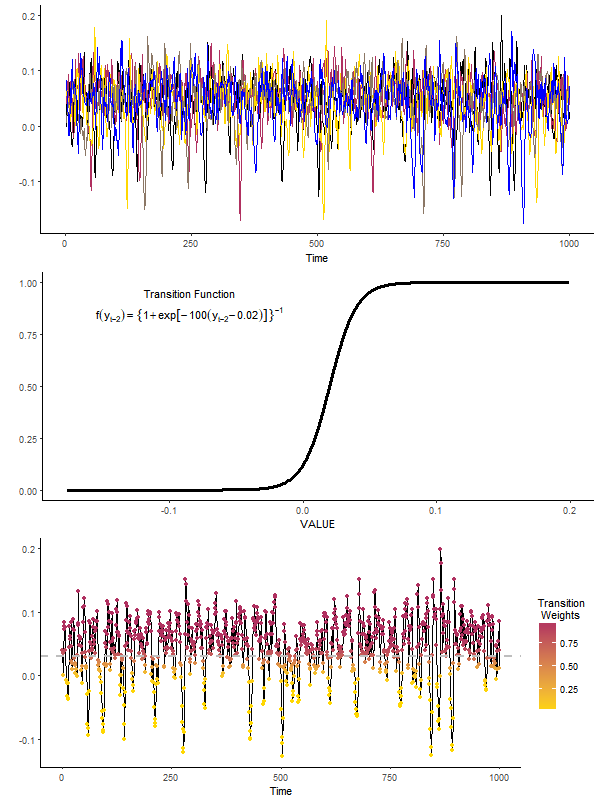
\includegraphics[scale=.7]{sim1plots}
	\label{fig:sim1plots}
\end{figure}

 This model is identical to the one presented in \cite{Lopes2006} where RJMCMC is used to select model order and a discrete $Uniform$ is adopted for $d$. If $p=4$ is known \textit{a priori}, the true parameter vector $\bm{\theta}=[\alpha_0, \alpha_1, \cdots, \alpha_4, \beta_0,\cdots,\beta_4, \gamma,\delta,\sigma]'$ contains $5$ zero parameters. Until further notice, $d$ is assumed to be known while the focus is on the ability of Bayesian shrinkage to combat over-fitting.

Bayesian estimation of the underlying LSTAR(2) model compares  BLASSO, RS-BLASSO, VS-BLASSO, and BHS shrinkage priors to conventional Normal priors. For the variations of BLASSO, posterior medians are obtained \citep{Park2008}, whereas when BHS \citep{Carvalho2009} or Normal priors are used, point estimates are based on posterior means. After a burn-in period of 15,000 and a thinning of 10 to reduce autocorrelation and control computer memory usage, 1,000 initial samples are obtained for 3 chains from the joint posterior distribution. The ``potential scale reduction factor'' (PSRF($\theta$)) of \cite{Gelman1992} evaluates convergence across the three chains, and effective sample size (ESS($\theta$)) measures mixing efficiency for each parameter $\theta \in \bm{\theta}$.  If $\underset{\theta}{\max} \textrm{ PSRF}(\theta)<1.05$ and $\underset{\theta}{\min} \textrm{ ESS}(\theta)>150$, convergence criteria is met and our initial sample is sufficient; otherwise, posterior samples are added, a maximum of 20 times, with intermittent convergence checks. Posterior simulations are only considered valid whenever the convergence criteria is met. Upcoming sections will follow the same convergence and reporting standards. Prior hyper-parameters are intentionally chosen to be non-informative and starting values are either randomly chosen or over-dispersed. Specifically for $\gamma^*$, a non-informative log normal prior $LN(3,1)$ is selected for all  simulation experiments \citep{Gerlach2008}. 

Table  \ref{tab:blassobhssummary} provides summary statistics of the posterior estimates from replications that converged using all five prior specifications. Rather than reporting the standard deviation of the estimates, estimation error is summarized using $RMSE(\theta)=\sqrt{\sum(\hat{\theta}-\theta)^2/n}$. There is consistent overestimation and large uncertainty for $\gamma$ --- commonly reported in literature \citep{Livingston2017} --- with the worst results for BHS and Normal priors. Figure \ref{fig:blvsbh} plots posterior estimates of the autoregressive parameters $\hat{\bm{\alpha}}$ and $\hat{\bm{\beta}}$. Discerning between shrinkage estimation methods is difficult since signal detection is satisfactory for all 4 methods. The optimal choice may be determined solely on computational efficiency which is left for discussion in a future subsection. Clearly, substantial improvements can be seen over the default normal prior choice.

\begin{sidewaystable}[htbp]
	\small
  \centering
  \caption{Posterior Estimate Summary for Simulation 1}
    \begin{tabular}{cccccccccccc}
    \toprule
   & & \multicolumn{2}{c}{BLASSO} &\multicolumn{2}{c}{RS-BLASSO} &\multicolumn{2}{c}{VS-BLASSO}  & \multicolumn{2}{c}{BHS} & \multicolumn{2}{c}{Normal} \\
    \cline{3-4} \cline{5-6} \cline{7-8} \cline{9-10} \cline{11-12}\\
    Parameter & Actual & Mean  & RMSE &  Mean & RMSE & Mean & RMSE & Mean & RMSE & Mean & RMSE   \\
    \midrule
   $\alpha_0$ & 0    & 0.0011 & 0.0024 & 0.0011 & 0.0025 & 0    & 0    & 0.0007 & 0.002 & 0.0049 & 0.0054 \\
    $\alpha_1$ & 1.8  & 1.7666 & 0.0715 & 1.7696 & 0.068 & 1.7765 & 0.0624 & 1.768 & 0.0746 & 1.5165 & 0.2898 \\
    $\alpha_2$ & -1.06 & -1.0046 & 0.1003 & -1.0108 & 0.0924 & -1.0367 & 0.081 & -1.0104 & 0.1159 & -0.5786 & 0.4888 \\
    $\alpha_3$ & 0    & -0.0042 & 0.0103 & -0.0026 & 0.0066 & 0.0007 & 0.0237 & -0.0125 & 0.0434 & -0.1745 & 0.1878 \\
    $\alpha_4$ & 0    & -0.004 & 0.0142 & -0.0027 & 0.0105 & -0.0022 & 0.0155 & -0.0028 & 0.031 & -0.0125 & 0.0618 \\
    $\beta_0$ & 0.02 & 0.0199 & 0.0039 & 0.0201 & 0.0067 & 0.0205 & 0.0032 & 0.0202 & 0.0035 & 0.021 & 0.0043 \\
    $\beta_1$ & 0.9  & 0.8714 & 0.0772 & 0.8697 & 0.1069 & 0.8987 & 0.0475 & 0.8899 & 0.0528 & 0.8635 & 0.0661 \\
    $\beta_2$ & -0.265 & -0.2246 & 0.0732 & -0.2253 & 0.0748 & -0.2684 & 0.0406 & -0.2496 & 0.053 & -0.2366 & 0.0584 \\
    $\beta_3$ & 0    & -0.0075 & 0.0139 & -0.0057 & 0.0114 & 0    & 0    & -0.0081 & 0.0296 & -0.0083 & 0.0504 \\
    $\beta_4$ & 0    & -0.0005 & 0.0151 & -0.0009 & 0.012 & -0.0003 & 0.0132 & 0.0019 & 0.0253 & 0.0033 & 0.0404 \\
    $\sigma$ & 0.02 & 0.0202 & 0.0004 & 0.0202 & 0.0004 & 0.0201 & 0.0004 & 0.0201 & 0.0004 & 0.021 & 0.0011 \\
    $\gamma$ & 100  & 131.0624 & 80.8034 & 131.5355 & 82.1307 & 131.0224 & 77.9754 & 174.15 & 148.8093 & 225.5381 & 204.5109 \\
    $\delta$ & 0.02 & 0.0218 & 0.0049 & 0.0218 & 0.0056 & 0.0204 & 0.0035 & 0.0208 & 0.0038 & 0.0261 & 0.0083 \\
    \bottomrule
    \end{tabular}%
  \label{tab:blassobhssummary}%
\end{sidewaystable}%

\begin{figure}[!h]
	\centering
	      \caption{Plot of $\hat{\bm{\alpha}}$ and $\hat{\bm{\beta}}$ for Simulation 1 }
      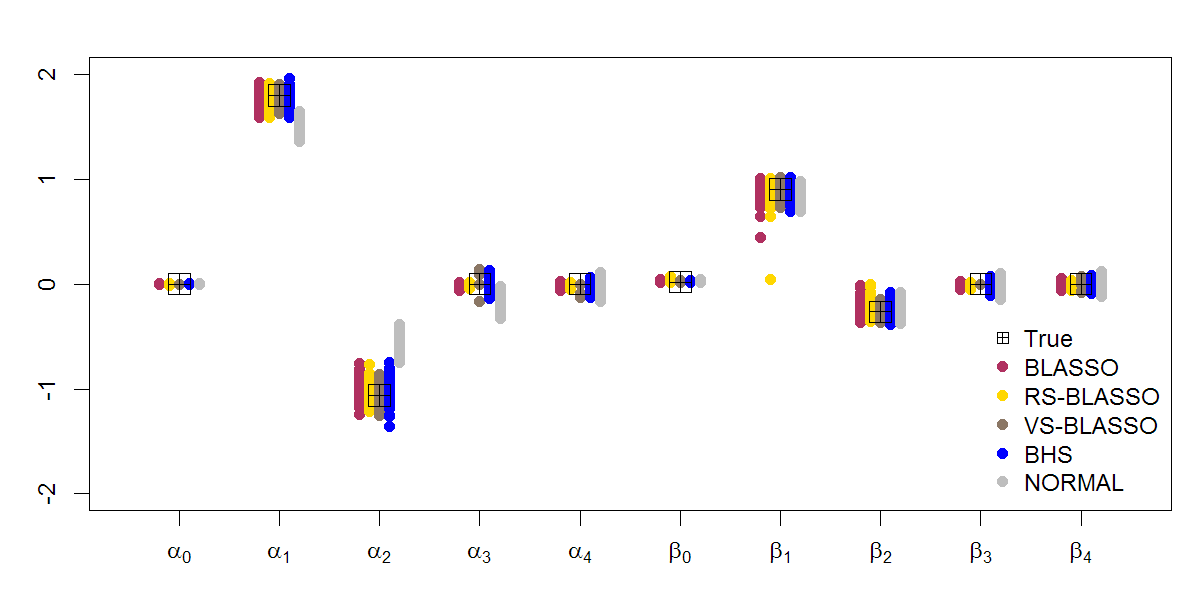
\includegraphics[scale=0.35]{blassovsbhs}
      \label{fig:blvsbh}
\end{figure}

Comparing our results to \cite{Lopes2006} is difficult for a number of reasons. For 50 replications, they obtain one MCMC chain of 2,500 posterior samples after a burn-in of 5,000; prior hyper-parameters are not specified and initial values are fixed. In this well-behaved case, posterior model probabilities pointed to the correct model 49 out of 50 times. For each replication, estimates are only based on the posterior samples where RJMCMC visited the correct LSTAR(2) model; no information is given on how many of the 2,500 posterior samples come from the correct parameter space. In \cite{Lopes2006}, overall summaries are based on the standard deviation (SD) of posterior estimates, whereas RMSE is evaluated here. The SD summarizes how much the posterior estimates differed from each other, while RMSE shows how much the posterior estimates differed from the truth. The main purpose for repeating this study is not to compare RJMCMC to Bayesian shrinkage but to establish the efficacy of these alternative methods for estimating a relatively simple LSTAR model. 

\subsection{Simulation 2: LSTAR with Gaps and Incremental Changes to Error Variance}
The next experiment is based on 100 replications of the LSTAR(3) model described in Equation \ref{eq:sim2}.
 \begin{equation}
	\begin{split}
		\label{eq:sim2}
		y_t&=(-0.6y_{t-3})[1-G(y_{t-1})] +(0.02+0.75y_{t-3})[G(y_{t-1})]+\epsilon_t\\
		& \textrm{where: } G(y_{t-1})=\bigg\{1+\exp\big[-120(y_{t-1}-0.02)\big]\bigg\}^{-1} \\
		&\textrm{ and }\epsilon_t \sim \textrm{i.i.d. }  N (0,0.02^2)\\
	\end{split}
\end{equation}

\begin{figure}
	\centering
	\caption{Ten Random Replications (top), Transition Function (middle), and Illustration of Regime-switching Behavior  for Simulation 2}
	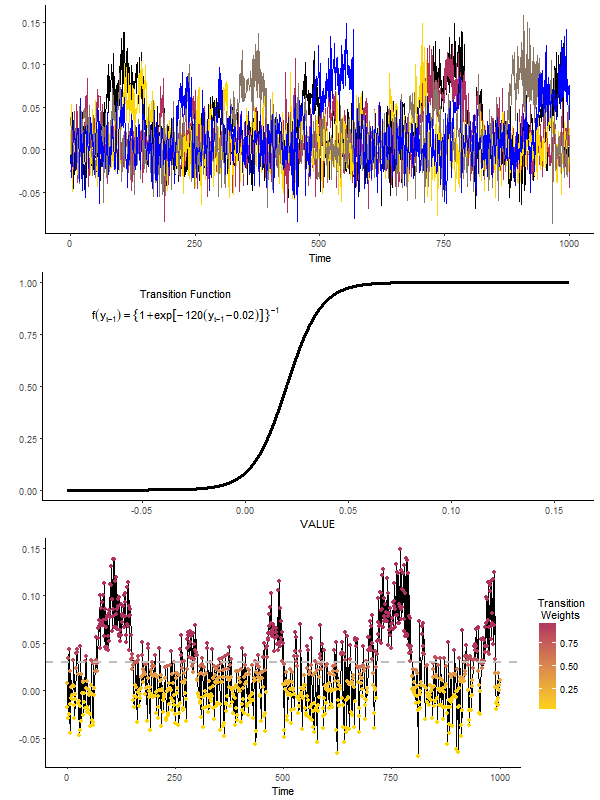
\includegraphics[scale=.7]{sim2plots}
	\label{fig:sim2plots}
\end{figure}

 Under the assumption that $p=4$, coefficients  $\bm{\theta}$ for autoregressive lags less than and larger than 3 are truly zero. This is a situation where even if RJMCMC visits the correct parameter space, normal priors will result in over-fitting. Motivation is geared towards nonlinear models where seasonal dynamics, of any period length, exhibit nonlinearities through dependence on some threshold variable.

Table \ref{tab:blassobhssummary3} summarizes and Figure \ref{fig:blvsbh3} illustrates the estimation accuracy of each method. Again, the normal priors result in unsatisfactory estimation accuracy. The simplest shrinkage methods, BLASSO and RS-BLASSO, consistently identify the true signal slightly better than the other shrinkage methods. 

\begin{sidewaystable}[htbp]
	\small
  \centering
  \caption{Posterior Estimate Summary for Simulation 2}
  \begin{tabular}{cccccccccccc}
    \toprule
   & & \multicolumn{2}{c}{BLASSO} &\multicolumn{2}{c}{RS-BLASSO} &\multicolumn{2}{c}{VS-BLASSO}  & \multicolumn{2}{c}{BHS} & \multicolumn{2}{c}{Normal} \\
    \cline{3-4} \cline{5-6} \cline{7-8} \cline{9-10} \cline{11-12}\\
    Parameter & Actual & Mean  & RMSE &  Mean & RMSE & Mean & RMSE & Mean & RMSE & Mean & RMSE   \\
    \midrule
    $\alpha_0$ & 0    & 0.0003 & 0.0011 & 0.0002 & 0.0011 & 0    & 0    & 0.0002 & 0.001 & 0.0041 & 0.0042 \\
    $\alpha_1$ & 0    & 0.0016 & 0.0097 & 0.0008 & 0.0051 & -0.0003 & 0.0157 & 0.0018 & 0.0273 & 0.2484 & 0.2556 \\
    $\alpha_2$ & 0    & 0.0004 & 0.007 & 0.0003 & 0.0041 & 0.0011 & 0.0094 & 0.0008 & 0.0154 & -0.0014 & 0.0517 \\
    $\alpha_3$ & -0.6 & -0.583 & 0.0547 & -0.5838 & 0.0544 & -0.5849 & 0.0548 & -0.5896 & 0.0537 & -0.2916 & 0.313 \\
    $\alpha_4$ & 0    & -0.0012 & 0.0073 & -0.0007 & 0.0044 & 0.0011 & 0.0075 & -0.0016 & 0.0149 & 0.0114 & 0.0529 \\
    $\beta_0$ & 0.02 & 0.0201 & 0.0019 & 0.0201 & 0.0018 & 0.0206 & 0.0021 & 0.0203 & 0.0021 & 0.0011 & 0.0195 \\
    $\beta_1$ & 0    & 0.0004 & 0.0051 & 0.0004 & 0.0044 & -0.0032 & 0.022 & -0.0022 & 0.0214 & 0.4269 & 0.4386 \\
    $\beta_2$ & 0    & 0.0005 & 0.0097 & 0.0006 & 0.0086 & 0.0016 & 0.0167 & 0.0002 & 0.0204 & 0.0008 & 0.0673 \\
    $\beta_3$ & 0.75 & 0.7307 & 0.046 & 0.73 & 0.0463 & 0.7306 & 0.0467 & 0.734 & 0.0439 & 0.5085 & 0.2764 \\
    $\beta_4$ & 0    & -0.0001 & 0.0067 & 0.0001 & 0.006 & -0.0004 & 0.0103 & -0.0012 & 0.0159 & -0.0113 & 0.0648 \\
    $\sigma$ & 0.02 & 0.0201 & 0.0004 & 0.0201 & 0.0004 & 0.0201 & 0.0004 & 0.02 & 0.0004 & 0.0232 & 0.0033 \\
    $\gamma$ & 120  & 130.5062 & 19.0649 & 130.3244 & 18.9201 & 128.4834 & 17.3982 & 130.9414 & 19.6161 & 686.7313 & 908.9353 \\
    $\delta$ & 0.02 & 0.0202 & 0.0013 & 0.0202 & 0.0013 & 0.0202 & 0.0013 & 0.0202 & 0.0013 & 0.025 & 0.007 \\
    \bottomrule
    \end{tabular}%
  \label{tab:blassobhssummary3}%
\end{sidewaystable}%

\begin{figure}[h]
	\centering
	      \caption{Plot of $\hat{\bm{\alpha}}$ and $\hat{\bm{\beta}}$ for Simulation 2}
      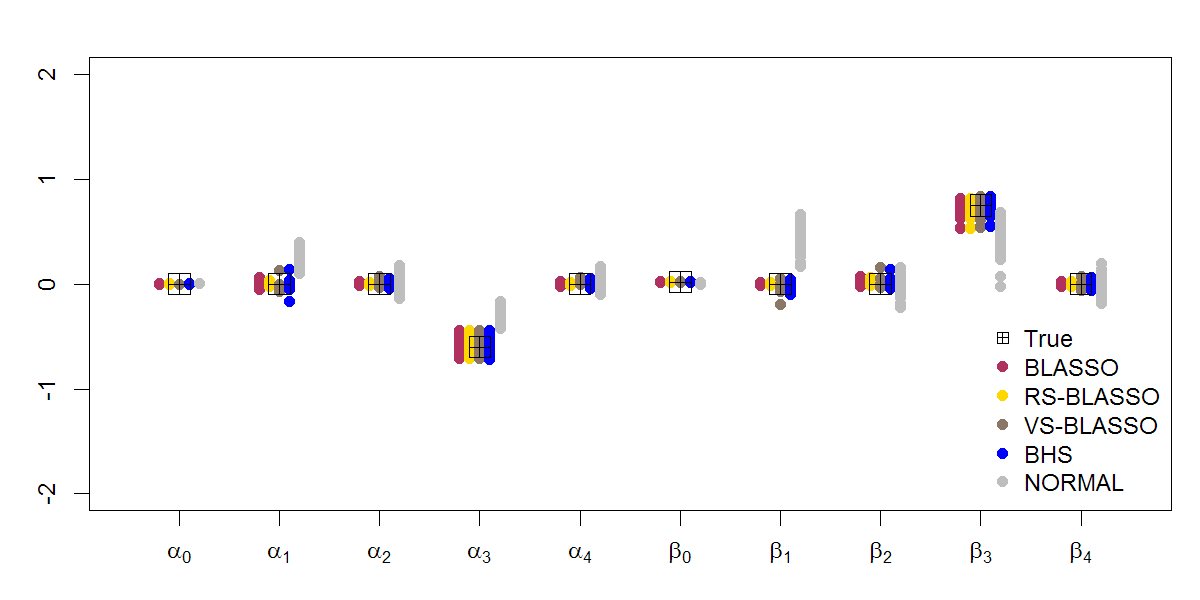
\includegraphics[scale=0.35]{blassovsbhs3}
      \label{fig:blvsbh3}
\end{figure}

Additionally, Simulation 2 is modified to allow $\sigma_k=0.02k$ $\forall k \in \{1,2,\cdots, 5\}$. For 50 replicates under each proposed $\sigma$, BLASSO and BHS methods are applied.  RMSE($\theta$) is naturally expected to increase with $\sigma$. The desire is to explore the sensitivity of RMSE($\theta$) as the noise is amplified. Under a fixed transition slope $\gamma=120$,  a contradictory trend was initially observed for known nonzero parameters $\alpha_3$ and $\beta_3$.  In Table \ref{tab:changingsigma}, RMSE($\alpha_3$) and RMSE($\beta_3$) gradually decline when $\gamma$ is fixed implying improved estimation. Increasing $\sigma$ naturally increases the sample standard deviation $s_{y}$. Under the reparameterization $\gamma=\gamma^*/s_y$, the unscaled transition slope $\gamma^*$ naturally must increase with $s_y$ to obtain the predetermined $\gamma=120$. 

Clearly, changing $\sigma$ has an impact on $\gamma^*$ through $s_y$. Although the actual transition function is not changing with $\sigma$ since it is fully determined by $\gamma$ and $\delta$, the speed of transition is increasing due to the natural modifications in the scope of the simulated data. The change is more visual in this regard. Therefore, for target $\gamma^*\approx 4$, data is simulated with $\gamma_k \approx 4/s_y$. Since $\sigma$ will naturally not equal $s_y$, the initial replications for each $\sigma_k$ under fixed $\gamma=120$ were used to obtain a mean estimate of $s_y$. Then, an appropriate $\gamma_k$ is determined for each $\sigma_k$, and 50 new replications are obtained. Table \ref{tab:changingsigma} shows the RMSE($\theta$) of each parameter for the specified options of $\sigma$ under fixed $\gamma_k=120$ and modified $\gamma_k$ to target $\gamma^*=4$. From these changes to the simulated data, RMSE($\alpha_3$) and RMSE($\beta_3$) increase with $\sigma_k$. Interestingly, the pattern for RMSE($\gamma$) is now reversed. These observations are  prevalent under both BLASSO and BHS priors; nevertheless, Bayesian shrinkage priors efficiently identify the nonlinear signal under gradual increases to the noise.




\begin{sidewaystable}[htbp]
\tiny
  \centering
  \caption{Sensitivity Analysis of RMSE($\bm{\theta}$) to $\sigma$ in Simulation 2}
    \begin{tabular}{cc|ccccc|ccccc}
    \toprule
    Method & Parameter & \multicolumn{5}{c}{Fixed Transition Slope} & \multicolumn{5}{c}{Modified Transition Slope} \\
    \midrule
    \multicolumn{2}{r|}{Choice of $\sigma$} & 0.02 & 0.04 & 0.06 & 0.08 & 0.1 & 0.02 & 0.04 & 0.06 & 0.08 & 0.1 \\
    \multicolumn{2}{r|}{Choice of $\gamma$} & \multicolumn{5}{c|}{$120$} & 109.60 & 71.47 & 49.50 & 37.46 & 30.02 \\
    \midrule
    BLASSO & $\alpha_0$ & 0.0009 & 0.0016 & 0.002 & 0.0025 & 0.0032 & 0.001 & 0.0016 & 0.0027 & 0.004 & 0.0049 \\
    & $\alpha_1$ &  0.0068 & 0.0104 & 0.0123 & 0.0145 & 0.013 & 0.0091 & 0.0141 & 0.0205 & 0.0248 & 0.0258 \\
    & $\alpha_2$ & 0.0125 & 0.0116 & 0.0102 & 0.0108 & 0.0102 & 0.0121 & 0.0136 & 0.0117 & 0.0127 & 0.0136 \\
    & $\alpha_3$ & 0.0479 & 0.0443 & 0.0383 & 0.0324 & 0.0328 & 0.0501 & 0.0522 & 0.055 & 0.0552 & 0.0543 \\
    & $\alpha_4$ & 0.0119 & 0.0128 & 0.008 & 0.0089 & 0.0106 & 0.012 & 0.0109 & 0.0097 & 0.0097 & 0.0099 \\
    & $\beta_0$ & 0.0019 & 0.0025 & 0.0038 & 0.0048 & 0.0059 & 0.0019 & 0.0027 & 0.0042 & 0.0057 & 0.0069 \\
    & $\beta_1$ & 0.006 & 0.0099 & 0.0152 & 0.0171 & 0.0177 & 0.0069 & 0.0066 & 0.0195 & 0.0227 & 0.0218 \\
    & $\beta_2$ & 0.0091 & 0.0147 & 0.0165 & 0.0154 & 0.0151 & 0.0127 & 0.0141 & 0.0154 & 0.0181 & 0.02 \\
    & $\beta_3$ & 0.0494 & 0.0429 & 0.0427 & 0.0438 & 0.0403 & 0.0579 & 0.061 & 0.0651 & 0.0683 & 0.0707 \\
    & $\beta_4$ & 0.008 & 0.0163 & 0.0136 & 0.0148 & 0.0204 & 0.0093 & 0.0202 & 0.0209 & 0.0195 & 0.0193 \\
    & $\sigma$ & 0.0005 & 0.0009 & 0.0014 & 0.0018 & 0.0023 & 0.0005 & 0.0009 & 0.0014 & 0.0018 & 0.0023 \\
    & $\gamma$ & 18.1887 & 23.4943 & 32.6301 & 32.8937 & 45.224 & 17.961 & 12.7347 & 9.5208 & 8.1114 & 7.1989 \\
    & $\delta$ & 0.0013 & 0.0019 & 0.0021 & 0.0025 & 0.0025 & 0.0013 & 0.0022 & 0.0038 & 0.0052 & 0.0065 \\
    \midrule
    HS & $\alpha_0$ & 0.0011 & 0.002 & 0.0028 & 0.0036 & 0.0049 & 0.0011 & 0.002 & 0.0033 & 0.0049 & 0.0065 \\
    & $\alpha_1$ & 0.0054 & 0.0127 & 0.0186 & 0.0236 & 0.0251 & 0.0063 & 0.0144 & 0.0233 & 0.03 & 0.0345 \\
    & $\alpha_2$ & 0.0075 & 0.013 & 0.0157 & 0.018 & 0.0181 & 0.0074 & 0.0141 & 0.0162 & 0.0192 & 0.0223 \\
    & $\alpha_3$ & 0.0485 & 0.0451 & 0.0386 & 0.0329 & 0.0334 & 0.0508 & 0.0545 & 0.0575 & 0.0576 & 0.0568 \\
   & $\alpha_4$ & 0.0079 & 0.0139 & 0.0138 & 0.0155 & 0.0174 & 0.008 & 0.0134 & 0.0159 & 0.0181 & 0.02 \\
    & $\beta_0$ & 0.0018 & 0.0024 & 0.0037 & 0.0046 & 0.0058 & 0.0018 & 0.0026 & 0.0039 & 0.0053 & 0.0067 \\
    & $\beta_1$ & 0.004 & 0.0111 & 0.0151 & 0.0204 & 0.0242 & 0.0039 & 0.0081 & 0.0162 & 0.022 & 0.0258 \\
    & $\beta_2$ & 0.0068 & 0.0152 & 0.0196 & 0.0214 & 0.0237 & 0.0071 & 0.014 & 0.0189 & 0.0226 & 0.0261 \\
   & $\beta_3$ & 0.0524 & 0.044 & 0.0442 & 0.0451 & 0.042 & 0.0608 & 0.0642 & 0.0688 & 0.072 & 0.0739 \\
    & $\beta_4$ & 0.0062 & 0.0164 & 0.0181 & 0.0215 & 0.0258 & 0.0063 & 0.0183 & 0.0227 & 0.024 & 0.0259 \\
    & $\sigma$ & 0.0005 & 0.0009 & 0.0014 & 0.0018 & 0.0023 & 0.0005 & 0.0009 & 0.0014 & 0.0018 & 0.0023 \\
   & $\gamma$ & 19.0596 & 24.0976 & 33.568 & 33.4267 & 45.3324 & 19.0212 & 13.5966 & 10.205 & 8.596 & 7.5575 \\
   & $\delta$ & 0.0013 & 0.0019 & 0.0021 & 0.0025 & 0.0025 & 0.0014 & 0.0022 & 0.0038 & 0.0052 & 0.0065 \\
    \bottomrule
    \end{tabular}%
  \label{tab:changingsigma}%
\end{sidewaystable}%


\subsection{Simulation 3: LSTAR with Regime-Specific Sparsity}

The effectiveness of the proposed methods is evaluated via simulating 100 replicates of the LSTAR(3) model in Equation \ref{eq:sim3}, exhibiting regime-specific complexity: the autoregressive dynamics are far simpler in the low regime relative to the high regime.
 \begin{equation}
	\begin{split}
		\label{eq:sim3}
		y_t&=(-0.7y_{t-3})[1-G(y_{t-1})] \\
		& +(0.06+0.4y_{t-1}-0.35y_{t-2}+0.2y_{t-3})[G(y_{t-1})]+\epsilon_t\\
		& \textrm{where: } G(y_{t-1})=\bigg\{1+\exp\big[-120(y_{t-1}-0.03)\big]\bigg\}^{-1} \\
		&\textrm{ and }\epsilon_t \sim \textrm{i.i.d. }  N (0,0.02^2)\\
	\end{split}
\end{equation}

\begin{figure}[ht!]
	\centering
	\caption{Ten Random Replications (top), Transition Function (middle), and Illustration of Regime-switching Behavior  for Simulation 3}
	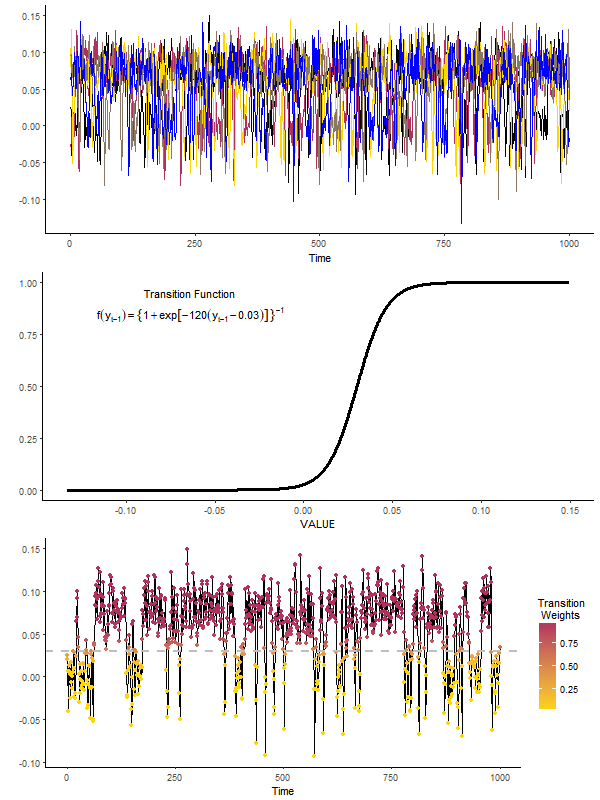
\includegraphics[scale=.7]{sim3plots}
	\label{fig:sim3plots}
\end{figure}
From Table \ref{tab:blassobhssummary4} and Figure \ref{fig:blvsbh4}, one observes that estimation accuracy is satisfactory for all three shrinkage methods, whereas $Normal$ priors continue to lead to poor estimates. The motivation for regime-specific shrinkage parameters $\lambda_1$ and $\lambda_2$ is illustrated in Figure \ref{fig:lambdabox}, which presents histograms of posterior median estimates for the tuning parameters of BLASSO vs RS-BLASSO. The visual disparity between $\lambda_1$ and $\lambda_2$ is a result of the regime-specific sparsity patterns: $\lambda_1>\lambda_2$ necessitates from the lower regime requiring relatively more shrinkage to identify the underlying signal.

\begin{sidewaystable}[htbp]
	\scriptsize
  \centering
  \caption{Posterior Estimate Summary for Simulation 3}
  \begin{tabular}{cccccccccccc}
    \toprule
   & & \multicolumn{2}{c}{BLASSO} &\multicolumn{2}{c}{RS-BLASSO} &\multicolumn{2}{c}{VS-BLASSO}  & \multicolumn{2}{c}{BHS} & \multicolumn{2}{c}{Normal} \\
    \cline{3-4} \cline{5-6} \cline{7-8} \cline{9-10} \cline{11-12}\\
    Parameter & Actual & Mean  & RMSE &  Mean & RMSE & Mean & RMSE & Mean & RMSE & Mean & RMSE   \\
    \midrule
   $\alpha_0$ & 0    & -0.0003 & 0.0019 & 0    & 0.0017 & 0    & 0.0003 & 0    & 0.002 & 0.0125 & 0.0126 \\
    $\alpha_1$ & 0    & 0.0011 & 0.0092 & 0.0003 & 0.0026 & -0.0004 & 0.0151 & 0.003 & 0.0431 & 0.6015 & 0.6135 \\
    $\alpha_2$ & 0    & -0.0031 & 0.0123 & -0.0006 & 0.0035 & -0.0035 & 0.0244 & -0.0058 & 0.0375 & -0.093 & 0.1118 \\
    $\alpha_3$ & -0.7 & -0.6785 & 0.0448 & -0.6816 & 0.0439 & -0.6754 & 0.052 & -0.6803 & 0.0553 & -0.4609 & 0.2483 \\
    $\alpha_4$ & 0    & -0.0016 & 0.0131 & -0.0005 & 0.0044 & -0.0008 & 0.0118 & -0.0026 & 0.0311 & -0.056 & 0.1002 \\
    $\beta_0$ & 0.06 & 0.0612 & 0.0046 & 0.0613 & 0.0042 & 0.061 & 0.0042 & 0.0609 & 0.0042 & 0.0301 & 0.0305 \\
    $\beta_1$ & 0.4  & 0.3692 & 0.0674 & 0.37 & 0.0613 & 0.3802 & 0.0545 & 0.3809 & 0.056 & 0.7792 & 0.3863 \\
    $\beta_2$ & -0.35 & -0.3054 & 0.0695 & -0.3005 & 0.0717 & -0.3292 & 0.0508 & -0.3242 & 0.0536 & -0.3312 & 0.0501 \\
    $\beta_3$ & 0.2  & 0.1597 & 0.0596 & 0.1538 & 0.0643 & 0.1844 & 0.0375 & 0.1766 & 0.0454 & 0.1371 & 0.0771 \\
    $\beta_4$ & 0    & 0.0104 & 0.0202 & 0.0101 & 0.0198 & 0.0015 & 0.0128 & 0.0063 & 0.0225 & -0.0087 & 0.039 \\
    $\sigma$ & 0.02 & 0.0202 & 0.0005 & 0.0202 & 0.0004 & 0.0201 & 0.0004 & 0.0201 & 0.0004 & 0.0239 & 0.0039 \\
    $\gamma$ & 120  & 120.5942 & 9.7438 & 121.8142 & 10.8705 & 121.3552 & 10.2547 & 123.1839 & 11.4902 & 617.4922 & 740.3125 \\
    $\delta$ & 0.03 & 0.0302 & 0.0011 & 0.0303 & 0.0011 & 0.0303 & 0.001 & 0.0302 & 0.0011 & 0.0378 & 0.0089 \\
    \bottomrule
    \end{tabular}%
  \label{tab:blassobhssummary4}%
\end{sidewaystable}%

\begin{figure}[!h]
	\centering
	      \caption{Plot of $\hat{\bm{\alpha}}$ and $\hat{\bm{\beta}}$ for Simulation 3}
      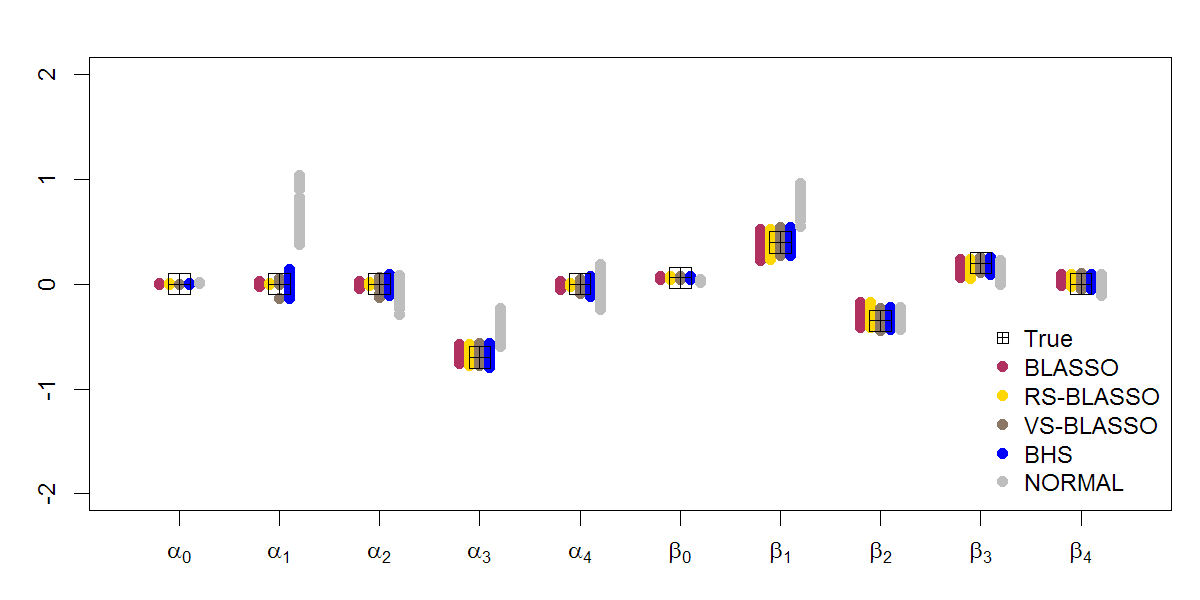
\includegraphics[scale=0.35]{blassovsbhs4}
      \label{fig:blvsbh4}
\end{figure}

\begin{figure}[!h]
	\centering
	      \caption{Posterior Shrinkage Comparison for BLASSO vs RS-BLASSO}
      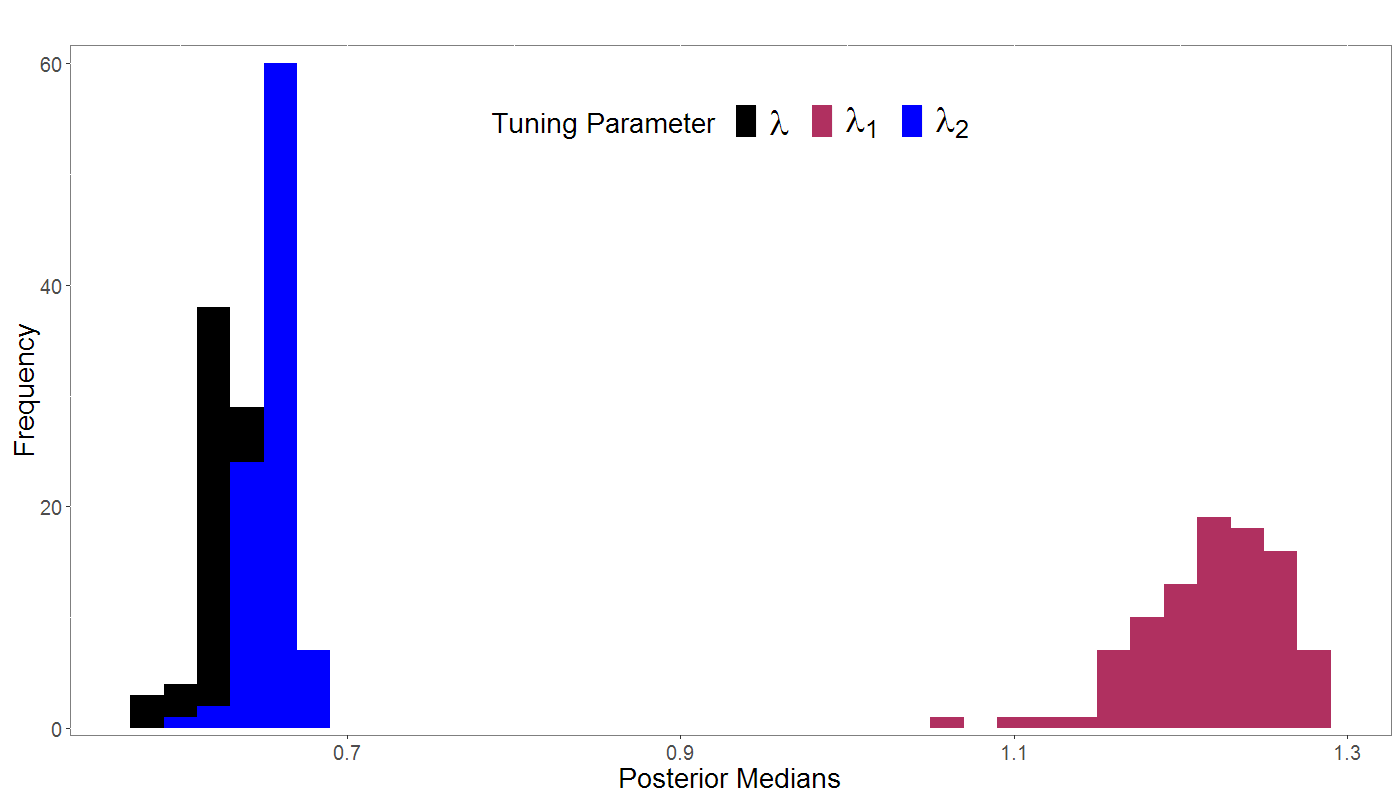
\includegraphics[scale=0.30]{rslambda}
      \label{fig:lambdabox}
\end{figure}

\vskip 3mm

\subsection{Convergence Analysis}

Simulations 1-3 were conducted on an Intel(R) Xeon (R) CPU E5-2697 v3 @ 2.60 GHz server with 132GB of RAM and 56 cores. Both the replications and the MCMC chains were parallel-processed within limitations of the server. The resources were often shared amongst colleagues, hence computational times can be misleading as a measure of efficiency. Since the parameter space is fixed for each MCMC routine, efficiency can be measured by the number of posterior samples required to attain the convergence criteria. Table \ref{tab:convtable} reports the percent of the 100 replications that converged along with the mean, median, and extreme percentiles of the samples required for the replications that converged.

When the model order $p$ is overestimated, the four shrinkage methods resist over-fitting to identify the true nonlinear process; therefore, choosing a method in practice ultimately depends on computational feasibility. All methods were equally efficient for Simulation 2 and unaffected by changes in noise. The methods were organized in order of regularization flexibility. For Simulations 1 and 3, the percent of converged replicates increased with the aforementioned flexibility. Specifically for Simulation 3, the additional tuning parameter in RS-BLASSO increased this percentage by 19\%, identifying the true advantage for regime-specific shrinkage. The BHS hierarchy is commended for being consistently efficient.

\begin{table}[!h]
\scriptsize
  \centering
  \caption{Convergence Statistics for Estimation Methods From Simulations 1-3}
    \begin{tabular}{cc|c|cccc}
    \toprule
    & & Percent of Replications & \multicolumn{4}{c}{Summary Statistics of Samples Required}\\
    Simulation & Method & Converged  & 5th Percentile   & Mean & Median & 95th Percentile \\
    \midrule
    1    & BLASSO & 91\%   & 1000 & 11615 & 2000 & 67000 \\
    1    & RS-BLASSO & 96\%    & 1000 & 10188 & 2000 & 110125 \\
    1    & VS-BLASSO & 99\%    & 1000 & 3202 & 2000 & 11000 \\
    1    & BHS  & 100\%   & 1000 & 1600 & 1000 & 4000 \\
    1    & Normal & 100\%   & 1000 & 1360 & 1000 & 4000 \\
    \midrule
    2    & BLASSO & 100\%   & 1000 & 1000 & 1000 & 1000 \\
    2    & RS-BLASSO & 100\%   & 1000 & 1000 & 1000 & 1000 \\
    2    & VS-BLASSO & 100\%   & 1000 & 2120 & 1000 & 4000 \\
    2    & BHS  & 100\%   & 1000 & 1010 & 1000 & 1000 \\
    2    & Normal & 100\%   & 1000 & 1150 & 1000 & 3050 \\
    \midrule
    3    & BLASSO & 75\%    & 1000 & 15800 & 2000 & 131500 \\
    3    & RS-BLASSO & 94\%    & 1000 & 1723 & 1000 & 4000 \\
    3    & VS-BLASSO & 100\%   & 1000 & 1380 & 1000 & 4000 \\
    3    & BHS  & 99\%    & 1000 & 1010 & 1000 & 1000 \\
    3    & Normal & 99\%    & 2000 & 8232 & 4000 & 46000 \\
    \bottomrule
    \end{tabular}%
  \label{tab:convtable}%
\end{table}%

\vskip 3mm

\subsection{Bayesian Selection of the Threshold Variable}

To incorporate the uncertainty for the delay $d$, Simulation 1 is revisited where the true threshold variable $y_{t-2}$ was assumed to be known. Maintaining the assumption $p = 4$, the vector $\bm{y}=[y_{t-1},y_{t-2},y_{t-3},y_{t-4}]'$ contains the threshold variables of interest. The re-paramaterized transition function $G(\bm{y})=\{1+\exp[-100(\bm{\phi}'\bm{y}-0.02)]\}^{-1}$ is equivalent to the transition function in Equation \ref{eq:sim1} when $\bm{\phi}=[\phi_1,\phi_2,\phi_3,\phi_4]'=[0,1,0,0]'$. Posterior sampling of $\bm{\phi}$ is combined with BLASSO and BHS under the previously stated convergence requirements. 

First, independent Bernoulli priors were used for $\phi_k$ along with BLASSO. Only 43\% of the replications converged compared to 91\% when $d=2$ was known. The average of the 43 posterior means for $\bm{\phi}$ was $[0.223,0.988,0.206,0.040]'$; the independent Bernoulli priors do not limit the threshold variable to one choice in  $\{y_{t-1},y_{t-2},y_{t-3},y_{t-4}\}$ since $\sum \phi_k \neq 1$ is not enforced. Estimation accuracy for non-$\bm{\phi}$ parameters was similar to the results presented in the previous Sections, but Bernoulli priors will not be discussed further due to computational deficiencies.

Next, let $\bm{\phi}\sim Dir([0.25,0.25,0.25,0.25]')$; the uninformative hyper-parameter demonstrates prior impartiality regarding $d$. BLASSO and BHS are combined with the $Dirichlet$ prior to re-estimate the 100 replications in Simulation 1, of which 98\% and 100\% converged, respectively. Table \ref{tab:rmsedirichlet} uses the RMSE of non-$\bm{\phi}$ parameters to show that MCMC sampling for $\bm{\phi}$ does not render the previous estimation methods useless. Table \ref{tab:estdirichlet} depicts summary statistics of the posterior means for $\bm{\phi}$ from the replications that converged. Figure \ref{fig:dirichlet1} overlays the posterior means summarized in Table \ref{tab:estdirichlet}. Both star plots heavily point toward the correct threshold variable indicating accurate estimation of $\bm{\phi}$. 
 
\begin{table}[!h]
	\footnotesize
  \centering
  \caption{Sensitivity of RMSE($\bm{\theta}$) to Uncertainty about $\bm{\phi}$ in Simulation 1}
    \begin{tabular}{cccccc}
    \toprule
    & \multicolumn{2}{c}{$\bm{\phi} \sim Dir$} & \multicolumn{2}{c}{$\bm{\phi}$ Known}\\
    \cline{2-3} \cline{4-5}
     Parameter & BLASSO & BHS & BLASSO & BHS  \\
    \midrule
    $\alpha_0$    & 0.0027 & 0.002 & 0.0024 & 0.002 \\
  $\alpha_1$  & 0.0763 & 0.0827 & 0.0715 & 0.0746 \\
    $\alpha_2$ & 0.1048 & 0.1269 & 0.1003 & 0.1159 \\
    $\alpha_3$    & 0.0103 & 0.038 & 0.0103 & 0.0434 \\
    $\alpha_4$    & 0.0153 & 0.0265 & 0.0142 & 0.031 \\
   $\beta_0$ & 0.0072 & 0.0034 & 0.0039 & 0.0035 \\
    $\beta_1$  & 0.1091 & 0.0541 & 0.0772 & 0.0528 \\
    $\beta_2$   & 0.0745 & 0.0549 & 0.0732 & 0.053 \\
   $\beta_3$     & 0.0147 & 0.0271 & 0.0139 & 0.0296 \\
    $\beta_4$    & 0.0156 & 0.0245 & 0.0151 & 0.0253 \\
   $\sigma$ & 0.0004 & 0.0004 & 0.0004 & 0.0004 \\
    $\gamma$  & 87.1606 & 91.2016 & 80.8034 & 148.8093 \\
    $\delta$ & 0.0058 & 0.004 & 0.0049 & 0.0038 \\
    \bottomrule
    \end{tabular}%
  \label{tab:rmsedirichlet}%
\end{table}%


\begin{table}[!h]
	\footnotesize
  \centering
  \caption{Posterior Estimate Summary for $\bm{\phi}$ in Simulation 1}
    \begin{tabular}{cccccccc}
    \toprule
    & & \multicolumn{3}{c}{BLASSO} & \multicolumn{3}{c}{ BHS} \\
    \cline{3-5} \cline{6-8}\\
   Parameter & Actual & 5th \%-ile   & Mean & 95th \%-ile   & 5th \%-ile   & Mean & 95th \%-ile \\
    \midrule
    $\phi_1$    & 0    & 0.0114 & 0.0557 & 0.1618 & 0.0110 & 0.0581 & 0.1920 \\
    $\phi_2$    & 1    & 0.6501 & 0.8686 & 0.9536 & 0.6008 & 0.8653 & 0.9527 \\
   $\phi_3$    & 0    & 0.0144 & 0.0465 & 0.1301 & 0.0143 & 0.0475 & 0.1254 \\
   $\phi_4$    & 0    & 0.0079 & 0.0292 & 0.0897 & 0.0082 & 0.0290 & 0.0810 \\
    \bottomrule
    \end{tabular}%
  \label{tab:estdirichlet}%
\end{table}%


\begin{figure}[!h]
\centering
\caption{Posterior Means of $\bm{\phi}$ for Simulation 1 Using BLASSO (left) and BHS (right)}
\begin{minipage}[h]{0.4\textwidth}
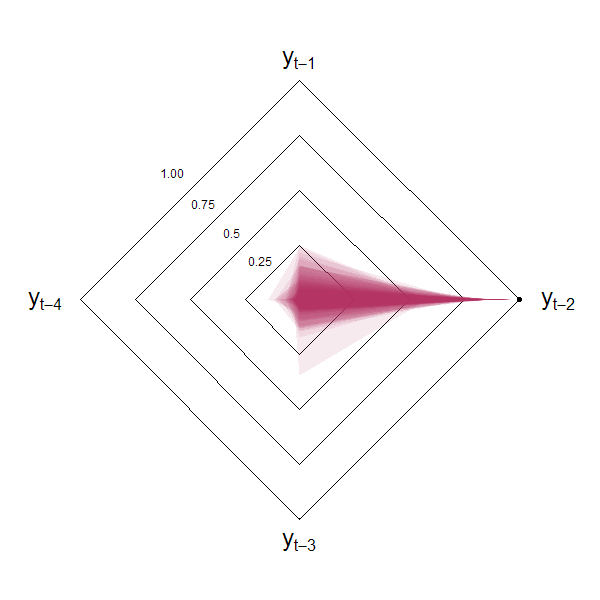
\includegraphics[scale=0.32]{blassodlp}
\end{minipage} \hspace{0.10\textwidth}
\begin{minipage}[h]{0.4\textwidth}
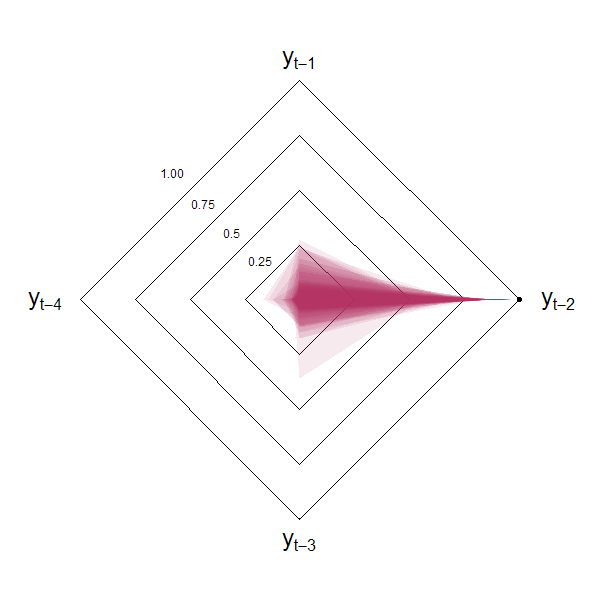
\includegraphics[scale=0.32]{hsdlp}
\end{minipage}
\label{fig:dirichlet1}
\end{figure}


Simulation 2 is repeated for three threshold variables denoted $z_{1,t},z_{2,t},$ and $z_{3,t}$ and identified in Equation \ref{eq:thvarchoice}. The first two threshold variables conform to the classic LSTAR structure; however, $z_{3,t}$ is an average of the first three lags of the endogenous time series $\bm{y_t}$. Conventional estimation of the delay $d$ would be unable to correctly identify $z_{3,t}$. Using BHS only, all 3 modifications are identifiable when a 4-dimensional $Dirichlet$ prior is used for $\bm{\phi}$.
 \begin{equation}
\label{eq:thvarchoice}
\begin{split}
	z_{1,t}&=y_{t-1}=\bm{\phi_1}'\bm{y}=[1,0,0,0]\bm{y}\\
	z_{2,t}&=y_{t-2}=\bm{\phi_2}'\bm{y}=[0,1,0,0]\bm{y}\\\
	z_{3,t}&=\frac{y_{t-1}+y_{t-2}+y_{t-3}}{3}=\bm{\phi_3}'\bm{y}=\bigg[\frac{1}{3},\frac{1}{3},\frac{1}{3},0\bigg]\bm{y}\\\
\end{split}
\end{equation}
Acknowledged uncertainty about the threshold variable manifests lower convergence rates than the original 100\% seen in Simulation 2. Based on 100 replications, convergence rates were 86\%, 75\%, and 87\% for  $z_{1,t}, z_{2,t},$ and $z_{3,t}$, respectively. For replications that converged, Figures 6-8 present posterior means of $\bm{\phi_k}$ for $k \in\{1,2,3\}$. Figure \ref{fig:th1} shows almost perfect posterior weighting towards the true $z_{1,t}=y_{t-1}$ while Figure \ref{fig:th2} provides evidence of occasional mis-identification of $z_{2,t}=y_{t-2}$. Figure \ref{fig:th3} for $z_{3,t}$ shows almost equal favor for $y_{t-1}$, $y_{t-2}$,  and $y_{t-3}$ while severely down-weighting $y_{t-4}$.

\begin{figure}[!h]
\center
\begin{minipage}[h]{0.4\textwidth}
\caption{Posterior Means of $\bm{\phi_1}$ When $z_{1,t}=y_{t-1}$}
\label{fig:th1}
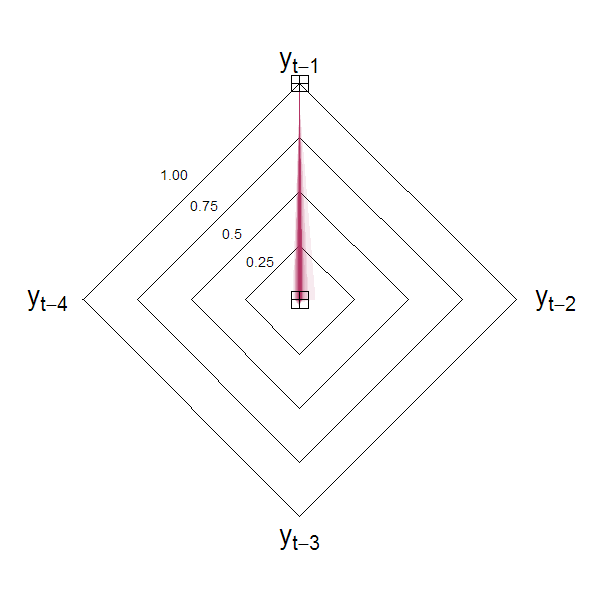
\includegraphics[scale=0.32]{hsthvar1}
\end{minipage} \hspace{0.1\textwidth}
\begin{minipage}[h]{0.4\textwidth}
\caption{Posterior Means of $\bm{\phi_2}$ When $z_{2,t}=y_{t-2}$}
\label{fig:th2}
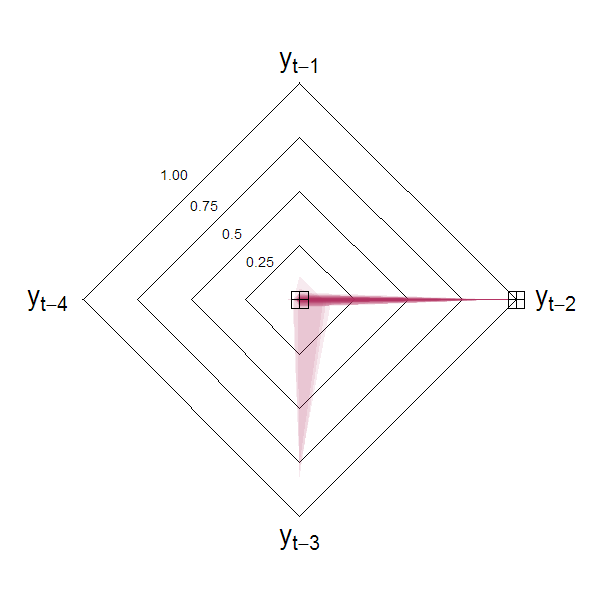
\includegraphics[scale=0.32]{hsthvar2}
\end{minipage}
\begin{minipage}[h]{0.8\textwidth}
\caption{Posterior Means of $\bm{\phi_3}$ When $z_{3,t}=\frac{y_{t-1}+y_{t-2}+y_{t-3}}{3}$}
\label{fig:th3}
\center
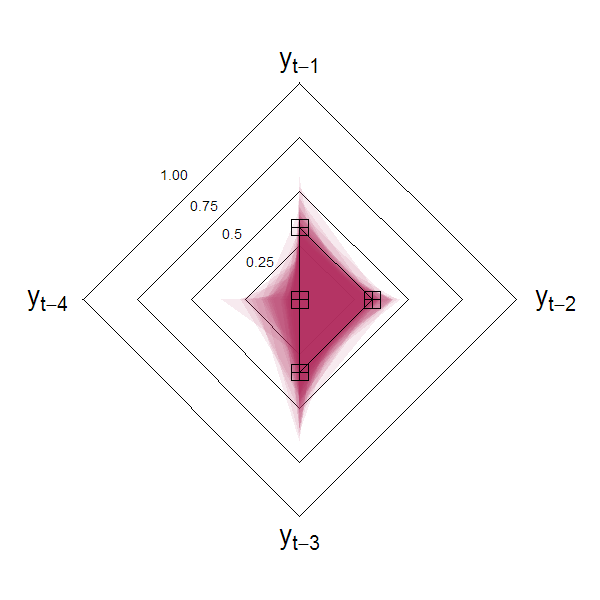
\includegraphics[scale=0.32]{hsthvar3}
\end{minipage}
\end{figure}


%%%%%%%%%%%%%%%%%%%%%%%%%%%%%%%%%%%%%%%%%%%%%%%%%%%%%%%%%%%%%%%


\section{Forecasting Annual Sunspot Numbers}

International sunspot numbers are gathered and updated by the World Data Center SILSO, Royal Observatory of Belgium, Brussels. Since \cite{Granger1957} , this data has served as an example in nonlinear time series literature. Letting $x_t$ represent the annual sunspot number at time $t$, the square root transformation $y_t= 2[\sqrt{1+x_t}-1]$ following \cite{Ghaddar1981} is applied. Data from 1700 to 1979 are used to estimate models while data from 1980 to 2006 are used to evaluate their forecasting accuracy. \cite{Terasvirta2010} compares three nonlinear time series models, namely STAR, TAR, and Artificial Neural Nets (AR-NN), to the baseline linear AR model. The LSTAR model in Equation \ref{eq:TModel} had optimal $h$-step ahead forecasting performance for horizons $h \in \{1,2,\cdots,5\}$. Sparsity is achieved through a stepwise frequentist procedure; henceforth, this model abbreviates to $F_T$. 
\begin{equation}
\begin{split}
 	y_t &=(1.46y_{t-1}-0.76y_{t-2}+0.17y_{t-7}+0.11y_{t-9})[1-G(y_{t-2},5.5,7.9)]\\
 	&+(2.7+0.92y_{t-1}-0.01y_{t-2}-0.47y_{t-3}+0.32y_{t-4}-0.26y_{t-5}\\
 	&+0.17y_{t-7}-0.24y_{t-8}+0.11y_{t-9}+0.17y_{t-10})G(y_{t-2},5.5,7.9)+\hat{\epsilon}_t\\
 	\textrm{where: } & \hat{\epsilon}_t \sim N(0, 1.898^2).\\
\end{split}
\label{eq:TModel}
\end{equation}
Simulation results indicate the difficulty of normal priors in combating over-fitting: even if RJMCMC directed to the correct model order $p=10$, current Bayesian approaches are incapable of estimating the model in Equation \ref{eq:TModel}. Assuming the delay $d=2$, a fully saturated LSTAR(10) model, denoted $F_S$, is estimated for a baseline comparison.

Hypothesis testing for the threshold variable produced ambiguous results as nonlinearity was rejected for multiple delay parameters. \cite{Terasvirta2010} chose $d=2$ based on p-value magnitude, but recommended LSTAR modeling for other values of $d$. Assuming $p=10$ and $d=2$, BHS priors estimate the LSTAR model, denoted $B_2$, in Equation \ref{eq:HSModel}. Posterior standard deviations are provided below the corresponding regime-specific AR coefficients. Parameter estimates for $\alpha_6$ and $\beta_6$ round to zero and are ignored from the model representation.
\begin{equation}
\begin{split}
 	y_t &=(-\underset{(1.14)}{0.56}+\underset{(0.20)}{1.56}y_{t-1}-\underset{(0.29)}{0.52}y_{t-2}+\underset{(0.15)}{0.01}y_{t-3}-\underset{(0.14)}{0.06}y_{t-4}\\
 	&-\underset{(0.12)}{0.03}y_{t-5} +\underset{(0.17)}{0.18}y_{t-7}+\underset{(0.13)}{0.05}y_{t-8}+\underset{(0.15)}{0.14}y_{t-9}-\underset{(0.10)}{0.04}y_{t-10})\\
 	&\times[1-G(y_{t-2},5.21,8.37)]+(\underset{(1.11)}{0.43}+\underset{(0.25)}{0.83}y_{t-1}+\underset{(0.28)}{0.14}y_{t-2}\\
 	&-\underset{(0.14)}{0.24}y_{t-3}+\underset{(0.11)}{0.06}y_{t-4}-\underset{(0.10)}{0.1}y_{t-5}
+\underset{(0.09)}{0.04}y_{t-7}-\underset{(0.14)}{0.13}y_{t-8}\\
&+\underset{(0.11)}{0.06}y_{t-9}+\underset{(0.10)}{0.14}y_{t-10})[G(y_{t-2},5.21,8.37)]+\hat{\epsilon}_t\\
 	\textrm{where: }  \hat{\epsilon}_t &\sim N(0, 1.94^2)\\
\end{split}
\label{eq:HSModel}
\end{equation}
Along with BHS priors, $\bm{\phi} \sim Dir ([\frac{1}{4},\frac{1}{4},\frac{1}{4},\frac{1}{4}]')$ for Bayesian estimation of the threshold variable $z_t=\bm{\phi}'\bm{y}$. Results from \cite{Terasvirta2010} indicate that $z_t \in \{y_{t-1},y_{t-2},y_{t-3},y_{t-4}\}$ is likely; therefore in the re-parameterization, let $\bm{y}=[y_{t-1},y_{t-2},y_{t-3},y_{t-4}]'$. The estimated model in Equation \ref{eq:HSModelDIR} provides conflicting results for $z_t$; this model is denoted $B_D$. Posterior mean of $\bm{\phi}$ places more weight on $y_{t-3}$ than the assumed threshold variable $y_{t-2}$.
\begin{equation}
\begin{split}
 	y_t &=(-\underset{(0.26)}{0.04}+\underset{(0.08)}{1.36}y_{t-1}-\underset{(0.12)}{0.55}y_{t-2}+\underset{(0.10)}{0.06}y_{t-3}-\underset{(0.08)}{0.01}y_{t-4}\\
 	&-\underset{(0.08)}{0.02}y_{t-5}-\underset{(0.09)}{0.02}y_{t-6}+\underset{(0.12)}{0.16}y_{t-7}+\underset{(0.09)}{0.03}y_{t-8}+\underset{(0.08)}{0.06}y_{t-9}\\
 	&+\underset{(0.05)}{0.02}y_{t-10})[1-G(z_t,31.87,9.66)]+(\underset{(0.48)}{0.18}+\underset{(0.08)}{0.91}y_{t-1}\\
 	&+\underset{(0.08)}{0.02}y_{t-2}-\underset{(0.08)}{0.07}y_{t-3}-\underset{(0.08)}{0.11}y_{t-5}+\underset{(0.06)}{0.01}y_{t-6}+\underset{(0.08)}{0.06}y_{t-7}\\
 	&-\underset{(0.09)}{0.07}y_{t-8}+\underset{(0.08)}{0.04}y_{t-9}+\underset{(0.06)}{0.06}y_{t-10})[G(z_t,31.87,9.66)]+\hat{\epsilon}_t\\
 	\textrm{where: }  z_t&=[0.16,0.15,0.62,0.08]\bm{y} \textrm{ and } \hat{\epsilon}_t \sim N(0, 1.88^2)\\
\end{split}
\label{eq:HSModelDIR}
\end{equation}
Using the \textit{Dirichlet} prior not only allows a compositional threshold variable, but can be used to shorten the list of possible lags. Under the assumption $d=3$, the estimated model ($B_3$) is seen in Equation \ref{eq:HSModel3}.
\begin{equation}
\begin{split}
 	y_t &=(\underset{(0.22)}{0.03}+\underset{(0.07)}{1.32}y_{t-1}-\underset{(0.11)}{0.6}y_{t-2}+\underset{(0.1)}{0.08}y_{t-3}+\underset{(0.09)}{0.06}y_{t-4}\\
 	&-\underset{(0.08)}{0.02}y_{t-5}-\underset{(0.09)}{0.04}y_{t-6}+\underset{(0.11)}{0.1}y_{t-7}+\underset{(0.09)}{0.05}y_{t-8}+\underset{(0.09)}{0.09}y_{t-9}\\
 	&+\underset{(0.05)}{0.03}y_{t-10})[1-G(y_{t-3},32.42,10.6)]+(\underset{(0.39)}{0.1}+\underset{(0.08)}{0.87}y_{t-1}\\
 	&+\underset{(0.08)}{0.03}y_{t-2}-\underset{(0.06)}{0.02}y_{t-3}+\underset{(0.07)}{0.01}y_{t-4}-\underset{(0.09)}{0.13}y_{t-5}-\underset{(0.06)}{0.01}y_{t-6}\\
 	&+\underset{(0.07)}{0.04}y_{t-7}-\underset{(0.08)}{0.05}y_{t-8}+\underset{(0.06)}{0.02}y_{t-9}+\underset{(0.05)}{0.04}y_{t-10})\\
 	&\times[G(y_{t-3},32.42,10.6)]+\hat{\epsilon}_t\\
 	\textrm{where: } \hat{\epsilon}_t &\sim N(0, 1.90^2)\\
\end{split}
\label{eq:HSModel3}
\end{equation}
The posterior standard deviations and means of autoregressive coefficients in models $B_2$, $B_D$, and $B_3$ suggest simpler LSTAR models than Terasvirta's in Equation \ref{eq:TModel}. Even simpler is the linear AR(10) model in Equation \ref{eq:LModel}, also estimated using BHS priors. Evidence of nonlinearity does not always guarantee that nonlinear specifications will outperform linear ones in forecasting accuracy\citep{Montgomery1998,Terasvirta2005}; thus the linear AR(10) model, denoted $B_{L}$ serves as a benchmark in the evaluation.
\begin{equation}
\begin{split}
 	y_t &=\underset{(0.64)}{0.83}+\underset{(0.06)}{1.22}y_{t-1}-\underset{(0.09)}{0.48}y_{t-2}-\underset{(0.09)}{0.08}y_{t-3}+\underset{(0.11)}{0.13}y_{t-4}\\
 	&-\underset{(0.09)}{0.1}y_{t-5}+\underset{(0.08)}{0.07}y_{t-7}-\underset{(0.09)}{0.07}y_{t-8}+\underset{(0.09)}{0.21}y_{t-9}+\underset{(0.06)}{0.03}y_{t-10}\\
 	\textrm{where: } \hat{\epsilon}_t &\sim N(0, 2.08^2)\\
\end{split}
\label{eq:LModel}
\end{equation}
Consistent with Terasvirta's textbook (2010), the evaluation is based on $h$-step ahead root mean squared forecast error ($RMSFE(h)$) for horizons $h \in \{1,2,\cdots,5\}$. Out-of-sample forecasts are obtained recursively using a rolling window without re-estimation. One-step ahead forecasts are directly obtainable. The nonlinear nature of LSTAR requires Monte Carlo sampling of the theoretical error distribution \citep{Peguin1994} or bootstrap sampling of the empirical error distribution for multi-step ahead forecasts \citep{Dijk2002,Lundbergh2002}. Robustness against distributional assumptions tilts favor toward bootstrapped forecasts \citep{Lin1994}. 

Table \ref{tab:ssrmsfe} compares $RMSFE(h)$ of the two frequentist  and four Bayesian estimated models. Models, $F_T$ and $B_2$, estimated under assumption $d=2$, perform clearly better than $B_D$ and $B_3$. This contradicts the evidence for $d=3$ seen in the training period. Efficacy of BHS shrinkage is illustrated through this extensively studied data: the best models, highlighted in bold, have almost identical forecasting performance for horizons 1 and 2, but $B_2$ starts outperforming at $h=3$. 

\begin{table}[!h]
	\small
  \centering
  \caption{$RMSFE(h)$ for Horizons $h \in \{1,2,\cdots,5\}$}
    \begin{tabular}{ccccccc}
    \toprule
     \multirow{2}[0]{*}{Model} & \multicolumn{5}{c}{Horizon} \\
                 & 1    & 2    & 3    & 4    & 5 \\
         \midrule
     $F_T$ &  {\bf 1.42} &  {\bf2}    &  {\bf2.36} &  {\bf2.51} & {\bf2.35} \\
            $F_S$ & 1.86 & 3.21 & 3.7  & 3.63 & 3.16 \\
         \midrule
       $B_L$ & 1.73 & 2.3  & 2.54 & 2.53 & 2.56 \\
        $B_2$ & {\bf 1.42} & {\bf1.96} &  {\bf2.29} &  {\bf2.19} & {\bf2.19} \\
         $B_D$ & 1.77 & 2.83 & 3.38 & 3.5  & 3.29 \\
          $B_3$ & 1.86 & 3.11 & 3.58 & 3.62 & 3.58 \\
    \bottomrule
    \end{tabular}%
  \label{tab:ssrmsfe}%
\end{table}%

%%%%%%%%%%%%%%%%%%%%%%%%%%%%%%%%%%%%%%%%%%%%%%%%%%%%%%%%%%%%%%%%%%%%%%%%

\section{Forecasting Daily Maximum Stream Water Temperatures}

\subsection{Background}

Climate change has been proven to have a negative effect on cold water species. As habitats become less suitable, the natural biodiversity in streams is altered. In a study of salmonid population in a mountain river network, rainbow trout migrated toward higher, colder elevations, while the bull trout significantly adjusted as the percent of the network suitable for habitation declined tremendously from 1993 to 2006 \citep{Isaak2010}. Furthermore, many nonnative invasive species inclined to warm water areas are infiltrating previously uninhabitable areas \citep{Rahel2008}. These distributional changes in streams alter localized food chains and thereby the entire ecosystem \citep{Albouy2014}. Letting $T_w(t)$ and $T_a(t)$ represent daily maximum water and air temperatures on day $t$, predictive models assist environmental authorities in assessing when water temperatures are expected to exceed certain species-specific thresholds.

\cite{Mohseni1998} exploited the S-curve shaped association between water and air temperatures using the nonlinear logistic model seen in Equation \ref{eq:equmod}. The lower asymptote $\beta_0$ represents the theoretical $\min T_w(t)$ and $\beta_1$ represents the theoretical range $\max T_w(t)- \min T_w(t)$. Parameters $\beta_2$ and $\beta_3$ control how fast water temperatures react to air temperature changes. The error term $E_t$ represents the deviation from the equilibrium profile at time $t$. 
\begin{equation}
	\label{eq:equmod}
	T_w(t)=\beta_0+\frac{\beta_1}{1+\exp[{\beta_2-\beta_3T_a(t)}]}+E_t
 \end{equation}
 
\cite{Caissie1998} employed harmonic regression models using Fourier series, to capture the annual cycles natural to water and air temperatures. The seasonality of daily maximum water and air temperatures is sufficiently captured by the first harmonic as seen in Equations \ref{eq:seasmod1} and \ref{eq:seasmod2}; the error terms $W_t$ and $A_t$ represent the deviations from seasonal maximum water and air temperature profiles at time $t$, respectively.
\begin{equation}
	\label{eq:seasmod1}
	T_w(t)=\beta_{0}+\beta_1\sin\bigg(\frac{2\pi t}{365.25}\bigg)+\beta_2\cos\bigg(\frac{2\pi t}{365.25}\bigg) + W_t
 \end{equation} 
 \begin{equation}
	\label{eq:seasmod2}
	T_a(t)=\beta_0+\beta_1\sin\bigg(\frac{2\pi t}{365.25}\bigg)+\beta_2\cos\bigg(\frac{2\pi t}{365.25}\bigg) + A_t
 \end{equation} 
The three river-specific profiles are estimated using historical data, and deviations are calculated. Instead of forecasting daily maximum water temperatures directly, models are designed to forecast deviations from the seasonal water temperature profiles. Let $\bm{w_t}=[W_{t},W_{t-1}, \cdots, W_{t-p_W}]'$, $\bm{a_t}=[A_t, A_{t-1}, \cdots, A_{t-p_A}]'$, and $\bm{e_t}=[E_t, E_{t-1}, \cdots, E_{t-p_E}]'$. Most commonly, subsets of the linear model seen in Equation \ref{eq:devmod} are employed in the literature \citep{Benyahya2007, Caissie2001}.
  \begin{equation}
	\label{eq:devmod}
	W_{t+1}=\mu+\bm{w_t}'\bm{\alpha} + \bm{a_t}'\bm{\beta} +  \bm{e_t}'\bm{\theta}+\epsilon_t
 \end{equation}
 
Previous research focused on forecasting 1-step ahead where subsets of the previous model perform competitively. Our interest is on 3-step and 7-step ahead forecasts; exploited nonlinearity may improve performance at longer horizons. The two exogenous time series, $A_t$ and $E_t$, complicate the multi-step ahead forecast of $W_{t+h}$, which not only depends on future unknown values $\{W_{t+1},W_{t+2},\cdots,W_{t+h-1}\}$ but also on both $\{A_{t+1},A_{t+2},\cdots,A_{t+h-1}\}$ and $\{E_{t+1},E_{t+2},\cdots,E_{t+h-1}\}$. The remedy is horizon-specific models where forecasting $W_{t+h}$, requires information at or before time $t$. For the basic LSTAR($p$) model, the iterative (Monte Carlo or bootstrap) approaches were shown to forecast better than this more direct approach on average \citep{Lin1994}. Nevertheless, computational advantages outweigh forecasting disadvantages, and horizon specific nonlinear models are seen throughout literature \citep{Stock1998a,Marcellino2006}.
 
Consider the three following horizon-specific models: Linear, shown in Equation \ref{eq:horizonspecificlinear}, nonlinear LSTAR with fixed threshold variable, depicted in Equation \ref{eq:horizonspecificnonlinear}, and nonlinear LSTAR with unknown threshold variable delineated in Equation \ref{eq:horizonspecificnonlineardir}. Given horizon $h$, the aforementioned specifications are respectively denoted $L(h)$, $N_1(h)$, and $N_2(h)$. Each model is developed from the same information and depends on the three model orders $p_W$, $p_A$, and $p_E$. Assumptions about the order parameters, such as $p_W=p_A=p_E=p$, simplify the MCMC sampling algorithm at a loss of model flexibility. 
  \begin{equation}
	\label{eq:horizonspecificlinear}
	W_{t+h}=\mu+\bm{w_t}'\bm{\alpha} + \bm{a_t}'\bm{\beta} +  \bm{e_t}'\bm{\theta}+\epsilon_t
 \end{equation} 
   \begin{equation}
   \begin{split}
	\label{eq:horizonspecificnonlinear}
	W_{t+h}&=(\mu_1+\bm{w_t}'\bm{\alpha_1} + \bm{a_t}'\bm{\beta_1} +  \bm{e_t}'\bm{\theta_1})[1-G(W_t,\gamma,\delta)]\\
	& + (\mu_2+\bm{w_t}'\bm{\alpha_2} + \bm{a_t}'\bm{\beta_2} +  \bm{e_t}'\bm{\theta_2})[G(W_t,\gamma,\delta)]+\epsilon_t\\
	\end{split}
 \end{equation}
     \begin{equation}
   \begin{split}
	\label{eq:horizonspecificnonlineardir}
	W_{t+h}&=(\mu_1+\bm{w_t}'\bm{\alpha_1} + \bm{a_t}'\bm{\beta_1} +  \bm{e_t}'\bm{\theta_1})[1-G(z_t,\gamma,\delta)]\\
	& + (\mu_2+\bm{w_t}'\bm{\alpha_2} + \bm{a_t}'\bm{\beta_2} +  \bm{e_t}'\bm{\theta_2})[G(z_t,\gamma,\delta)]+\epsilon_t\\
	& \textrm{where: } z_t=\bm{\phi}'\bm{w_t}\\
	\end{split}
 \end{equation}
 
 
 
 
 \vskip 3mm
 
 \subsection{The Data} 
 
Four years of daily maximum water temperatures and maximum air temperatures were collected from 31 rivers in Spain. The Spanish Environmental Department is credited for the water temperatures and the Spanish Meteorological Agency is credited for the air temperatures. Pairs of measurement stations were chosen for each river under strict guidelines to limit the impact from dams, cities, and fuel/nuclear power stations. The full data set is not limited to just daily maximum water and air temperatures; for further information, see \cite{Kamarianakis2016}.
 
For each river, the four years of data could come from any of the years between 2000 and 2008, inclusive. Typically the four years are often not consecutive and 15\% of the data is missing across all the rivers. To evaluate forecasting performance of river-specific linear and nonlinear models, the four years are split into a training and testing set. The training set contains the two, ideally consecutive, years of data with the least amount of missing observations. The two remaining years in the testing set typically are not adjacent and not immediately preceding the training period. 

\vskip 3mm

\subsection{Results}

For all 31 rivers, BHS priors result in sparse estimation of river specific models $L(h)$, $N_1(h)$, and $N_2(h)$ for $h \in \{3,7\}$. The maximum complexity considered is constrained by the assumption that $p=\max \{p_W, p_A, p_E\}=6$. Table \ref{tab:convriv} shows the percent of times the six models converged across the 31 rivers. Forecasting results from models where convergence was not reached after 20 updates are ignored. Models designed for horizon $h$ are evaluated based on their corresponding $RMSFE(h)$.

\begin{table}[!h]
	\small
  \centering
  \caption{ Percentages of River-Specific Models that Achieved Convergence }
    \begin{tabular}{ccc}
    \toprule
    &  \multicolumn{2}{c}{Horizon}  \\
    Model & 3 & 7\\
    \midrule
    $L(h)$ &  100\% & 97\%\\
    $N_1(h)$ & 97\% & 100\%\\
    $N_2(h)$ & 70\% & 81\%\\
    \bottomrule
    \end{tabular}%
  \label{tab:convriv}%
\end{table}%

Horizon specific linear models $L(3)$ and $L(7)$ outperform nonlinear alternatives for 67\% and 55\% of the rivers, respectively. 
When the nonlinear models outperform, the advantage is often marginal and insignificant. In these cases, the simpler linear specifications are more practical and therefore recommended. Now the focus is on three scenarios where the improvement from the nonlinear model was unusual relative to the rest of the rivers.

For Guadiana River, model $N_2(7)$ reduced overall RMSFE(7) by $0.098 \textrm{ }^o C$. Based on posterior weights $0.423$ and $0.301$, the threshold variable is approximately an average of $W_{t}$ and $W_{t-6}$, respectively and the estimated threshold is $0.06 \textrm{ }^o C$. Figures \ref{fig:gua1}-\ref{fig:gua2} show the posterior means of regime-specific autoregressive coefficients. In both regimes, the majority of information needed to forecast $W_{t+7}$ comes from the known seasonal deviation $W_t$; this phenomenon is stronger in the high regime.

\begin{figure}[!h]
\center
\begin{minipage}[h]{\textwidth}
\caption{Low Regime Coefficients for Guadiana from $N_1(7)$}
\label{fig:gua1}
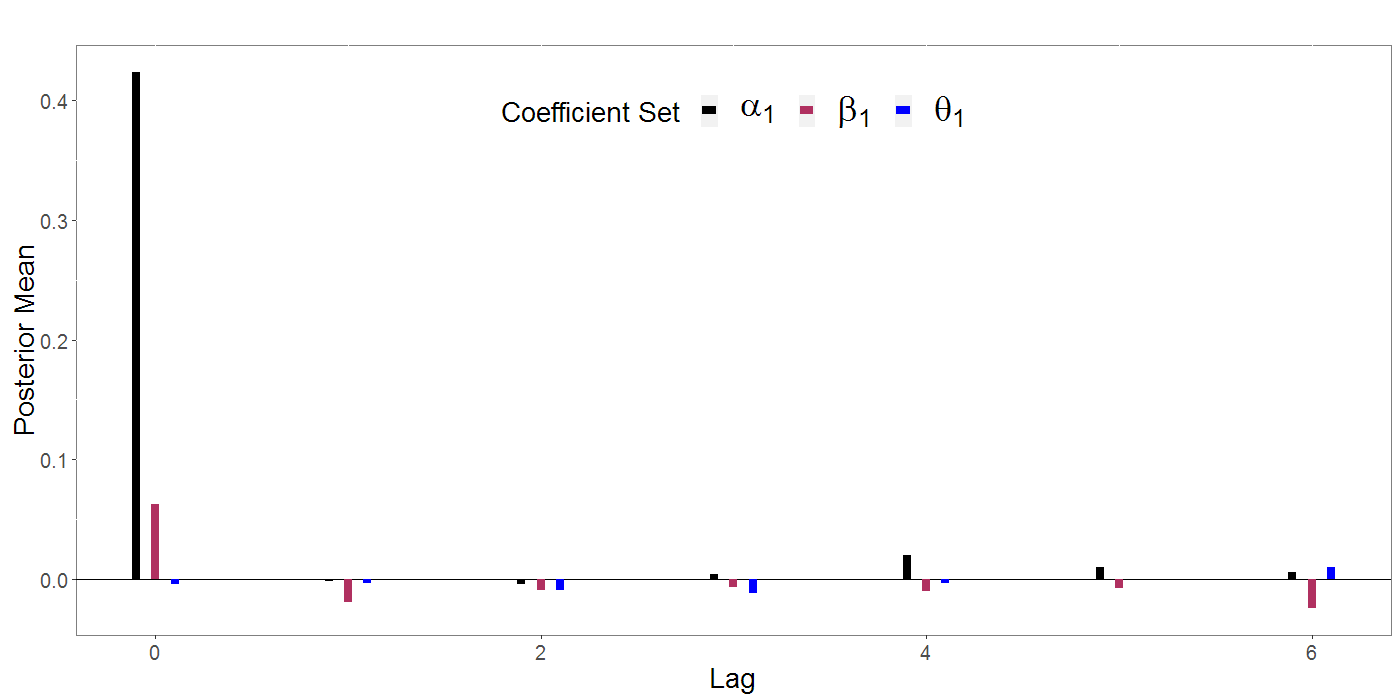
\includegraphics[scale=0.3]{GuadianaL}
\end{minipage} \hspace{\textwidth}
\begin{minipage}[h]{\textwidth}
\caption{High Regime Coefficients for Guadiana from $N_1(7)$}
\label{fig:gua2}
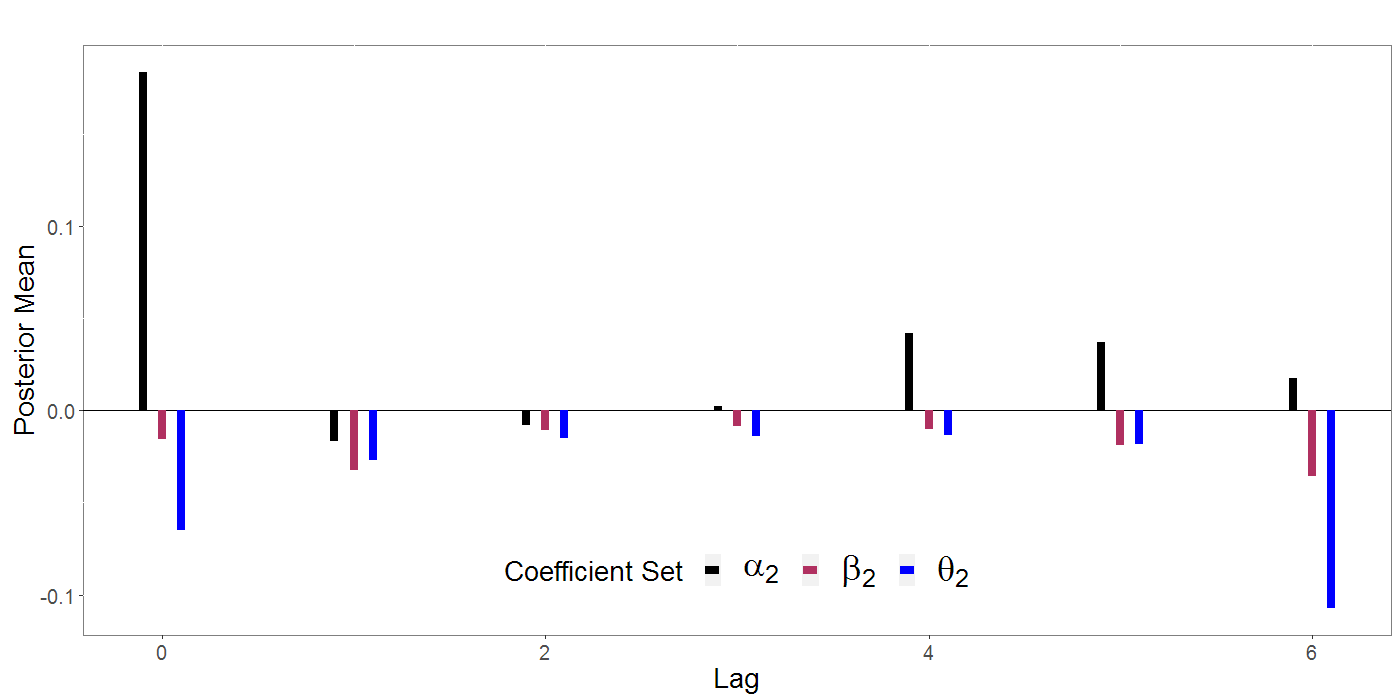
\includegraphics[scale=0.3]{GuadianaH}
\end{minipage}
\end{figure}


The next two examples involve the Jarama River where nonlinear models provided superior performance. For $h=3$, $N_2(3)$ reduced $RMSFE(3)$ by  $0.165 \textrm{ }^o C$; and for $h=7$, $N_1(7)$ reduced $RMSFE(7)$ by $0.105 \textrm{ }^o C$. Posterior expectations of $\bm{\alpha}$, $\bm{\beta}$, and $\bm{\theta}$ for $N_2(3)$ are shown in Figures \ref{fig:jar3}-\ref{fig:jar4} and for $N_1(7)$ are depicted in Figures \ref{fig:jar1}-\ref{fig:jar2}. For Jarama, it is intriguing that the optimal nonlinear model differs for the two horizons. The threshold variable in $N_2(3)$ places its largest weight of $0.66$ on $W_{t-6}$, representing information one week prior. These nonlinear models change dynamics around different thresholds: for $N_2(3)$, regime switching occurs when maximum water temperature at time $t$ surpasses its seasonal average at time $t$ by $1.20 \textrm{ }^o C$; and for $N_1(7)$, this change occurs for $0.65 \textrm{ }^o C$. The nonlinear dynamics exhibited in the low and high regimes also change with the horizon $h$. When forecasting $W_{t+3}$, the realization $W_t$ provides the most information when in the low regime; but in the high regime, none of the known information up to time $t$ is helpful. The model for forecasting $W_{t+7}$ is even more interesting since the AR dynamics in both regimes are similar to the high regime of $N_2(3)$. Knowing information at time $t$, specifically $W_t$, is only helpful in determining when to jump between means $\mu_L=0.002$ and $\mu_H=0.03$ to forecast 7-steps ahead. Obvious differences between these two horizon-specific models illustrate that for longer horizons, currently known data provide less useful information in forecasting.

\begin{figure}[!h]
\center
\begin{minipage}[h]{\textwidth}
\caption{Low Regime Coefficients for Jarama from $N_1(3)$}
\label{fig:jar3}
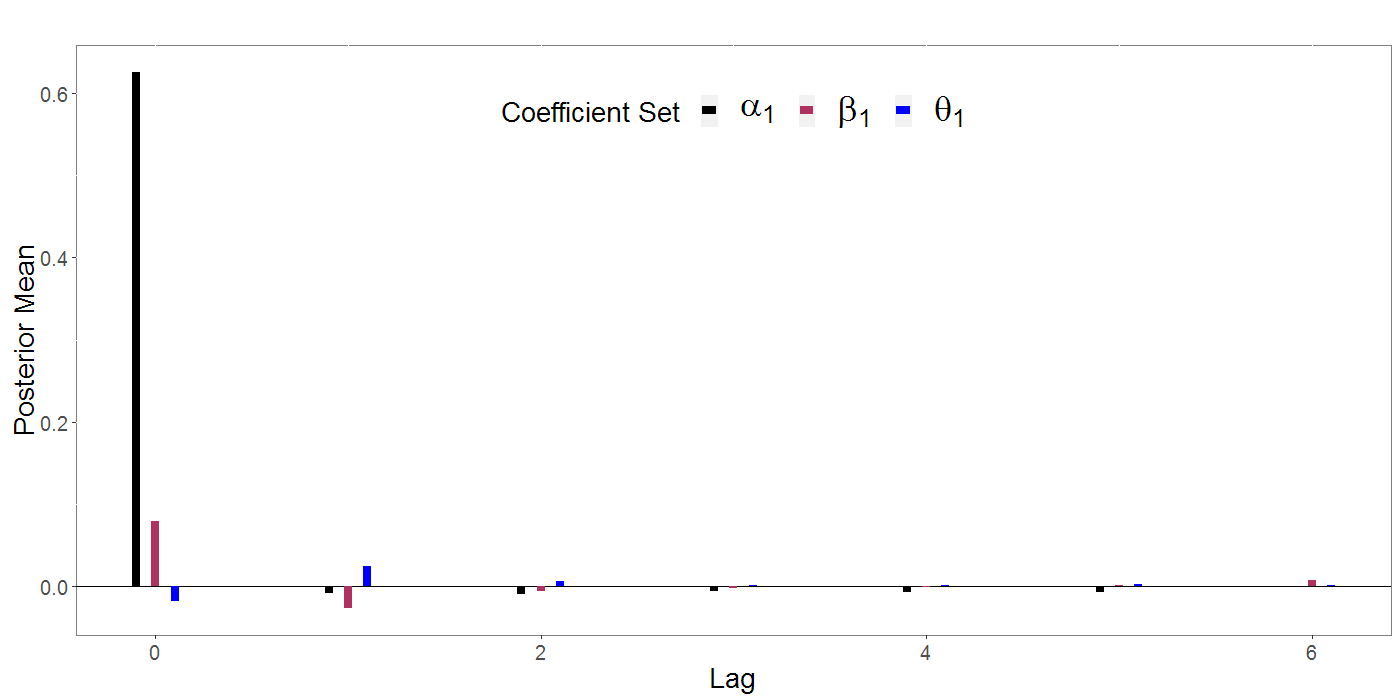
\includegraphics[scale=0.3]{JaramaL3}
\end{minipage} \hspace{\textwidth}
\begin{minipage}[h]{\textwidth}
\caption{High Regime Coefficients for Jarama from $N_1(3)$}
\label{fig:jar4}
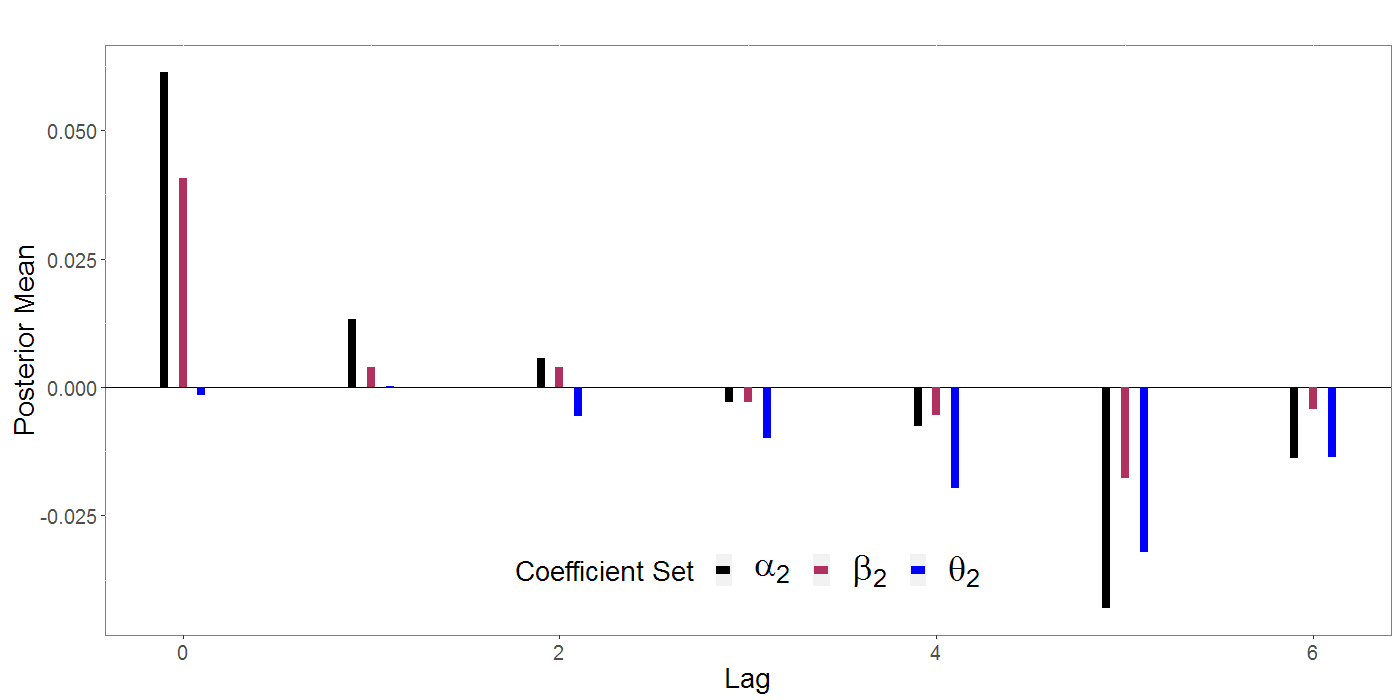
\includegraphics[scale=0.3]{JaramaH3}
\end{minipage}
\end{figure}

\begin{figure}[!h]
\center
\begin{minipage}[h]{\textwidth}
\caption{Low Regime Coefficients for Jarama from $N_1(7)$}
\label{fig:jar1}
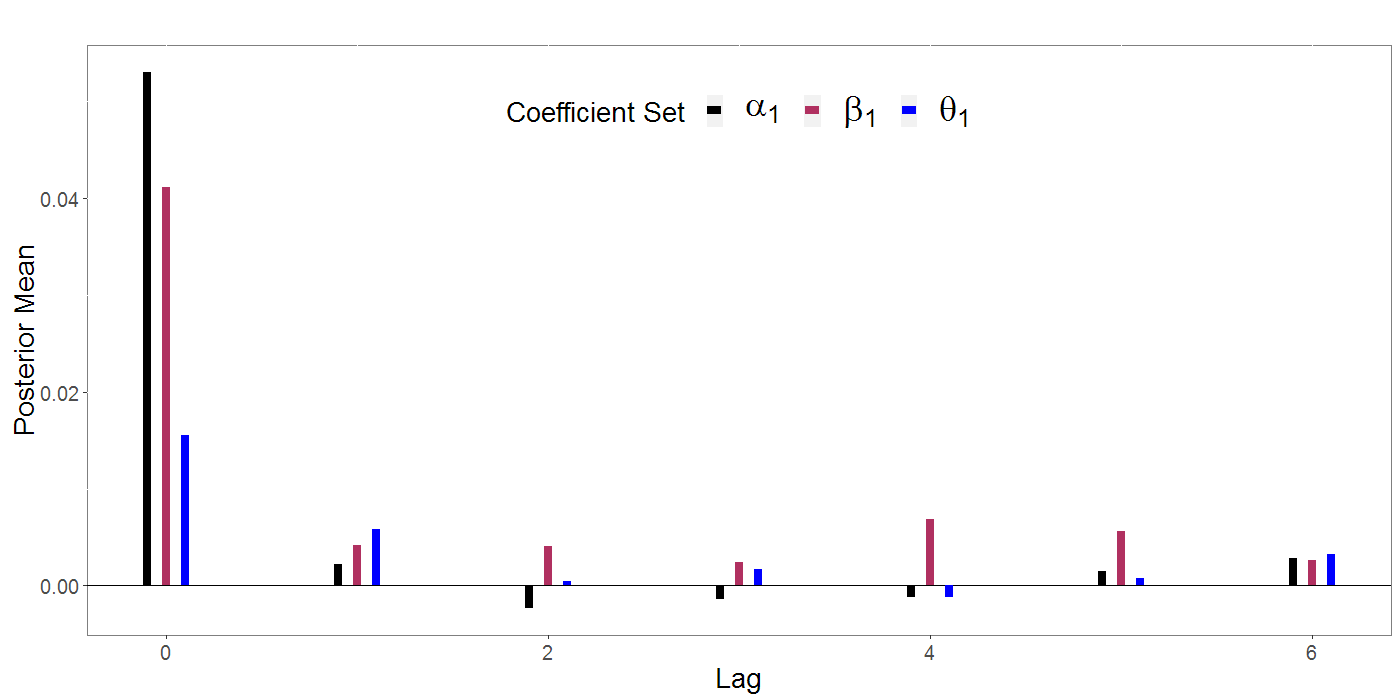
\includegraphics[scale=0.3]{JaramaL}
\end{minipage} \hspace{\textwidth}
\begin{minipage}[h]{\textwidth}
\caption{High Regime Coefficients for Jarama from $N_1(7)$}
\label{fig:jar2}
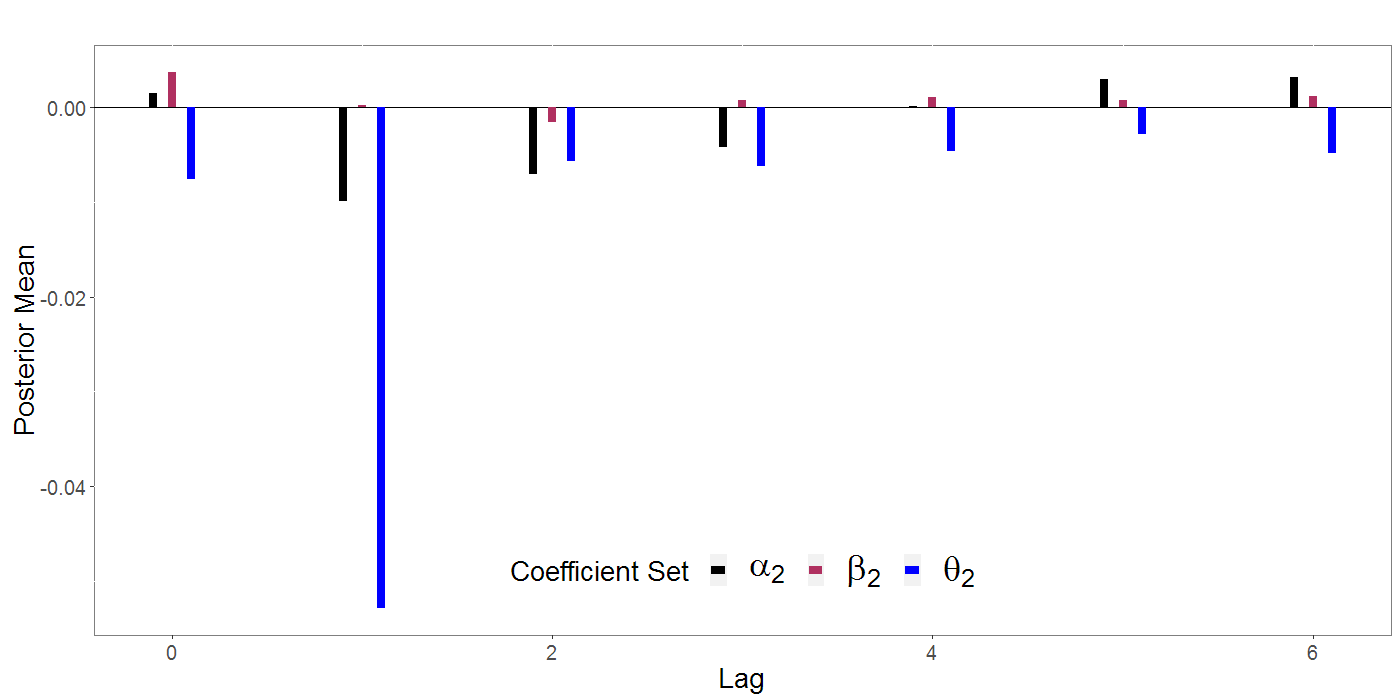
\includegraphics[scale=0.3]{JaramaH}
\end{minipage}
\end{figure}

\section{Conclusion}

Bayesian shrinkage priors for the AR coefficients and the \textit{Dirichlet} prior for a composite threshold variable are employed to estimate a flexible specification that nests the classic LSTAR model. Although simulation experiments show \textit{Dirichlet} priors to be an adequate alternative for estimating composite threshold variables, improved forecasting performance is not guaranteed. An advantage of the proposed methods is that practitioners can immediately apply them using common statistical software. Detailed code is provided with this paper for a tutorial in using Bayesian horseshoe to estimate nonlinear LSTAR models.

Recent alternatives to BLASSO and BHS based on the \textit{double-Pareto} \citep{Armagan2013} and \textit{Dirichlet-Laplace} priors \citep{Bhattacharya2015} may also be employed to estimate regime-specific autoregressive terms. Besides the jump from a linear to nonlinear LSTAR, which more than doubles the number of estimated parameters, increasing the assumed autoregressive orders in the regimes and the compositional threshold variable, further expands the parameter space causing slower convergence. For these reasons, a modified horseshoe representation is recommended for extremely sparse signals \citep{Bhadra2016}. 

The proposed methods can be easily employed to estimate nonlinear models represented by Equation \ref{eq:1} such as ESTAR and TAR. Future work involves applying and evaluating these methods on multiple regime smooth transition autoregressions (MR-STAR) where the number of unknown parameters may increase dramatically. For MR-STAR, Bayesian shrinkage may be used to circumvent the necessity for nested RJMCMC routines for each regime, or restrictive prior assumptions.

Sample code for this paper is provided in Appendix \ref{appendix1}. Code provides tutorial for implementing Bayesian regime-specific shrinkage estimation for nonlinear LSTAR models. Examples are provided in terms of a simulation study and an applied situation involving the monthly international sunspot numbers. The simulation study involving the composite threshold variable is used to illustrate the applicability and ease of the \textit{Dirichlet} prior. Code also pertaining to multistep ahead forecasts using the bootstrap method can prove to be useful in countless other situations outside the scope of this paper.

